%% ============================================================
%% SECTION: Results and Discussions
%% ============================================================

\section{Results and Discussions}

This adaptive scheme enables a balanced optimization process, starting with robust class-level discrimination and gradually shifting toward maximizing spatial overlap between predicted and ground truth tumour regions.

\subsection{Experimental Setup}

\subsubsection{Data Pre-processing and Training}

For Training we have used the Data from the popular BraTS Dataset, modifying it slightly to our convenience. In the BraTS Dataset, each image consists of four modalities. These modalities are essentially different representations of the same brain image but containing different types of information as they are captured through different criterion. These modalities are called T1, T1CE(T1 Contrast Enhanced), T2, and Flair. All the modalities for each date are present in the dataset in the form of .nii flies, along with the ground-truth mask which is also present in .nii file format. For processing this data prior to training we excluded the T1 modality, as T1CE is just the contrast enhanced version of T1, as it contains most of the information present in T1 while additionally providing contrast-enhanced information due to it being contrast enhanced. This means we can reduce 25\% size for each data while loosing little to no useful information. For the remaining 3 modalities(T1CE, T2 and Flair) we first cropped each modality from a size of $240\times240\times155$ to $128\times128\times128$. Now theoretically this may also lead to loosing so essential information from the data. However, even after hard cropping, we still retain almost all the image information. This is shown in Fig.~\ref{fig:wide}

\begin{figure*}[!htbp]
    \centering

    \begin{subfigure}[b]{0.48\textwidth}
        \centering
        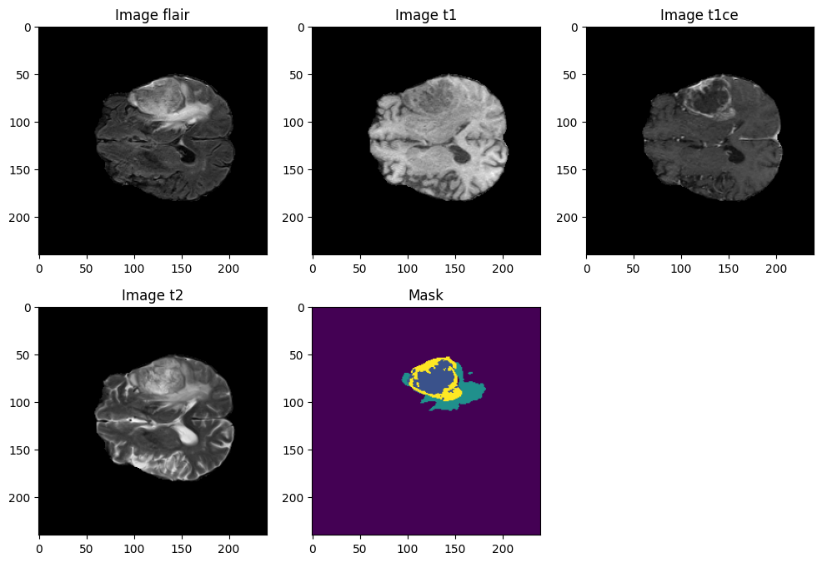
\includegraphics[width=\linewidth]{figs/Dataset Prep Img1.png}
        \caption{Uncropped Data}
        \label{fig:segA}
    \end{subfigure}
    \hfill
    \begin{subfigure}[b]{0.48\textwidth}
        \centering
        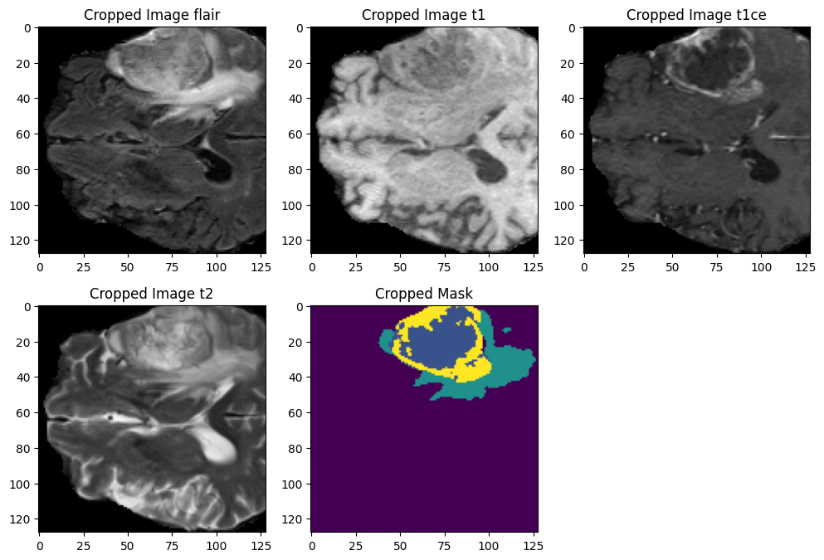
\includegraphics[width=\linewidth]{figs/Dataset Prep Img2.png}
        \caption{Cropped Data}
        \label{fig:segB}
    \end{subfigure}

    \caption{Visual comparison demonstrating the impact of cropping in the worst-case scenario, namely at the middle slice where the brain occupies its maximum cross-sectional area.}
    \label{fig:wide}
\end{figure*}

In this we are seeing exactly the middle slice of an example data. Being the middle slice, this is the worst case scenario of how the crop affects the data, as the brain cannot be any wider in any other portion. As even in the widest part of the brain more than 90\% of the data is still present, and almost all off the ground truth mask is present. This suggests that that >97\% of the useful data is still present. Through cropping, we are discarding the black empty portion around the brain, making the date more light weight and easier to handle. this trade-off was considered acceptable due to the negligible impact on segmentation performance as even if we feed the model uncropped data afterwords when the training is done, it predicts the ground truth mask with effectively the same accuracy. This cropping strategy was also beneficial as it brings the size of each dimension in the order of $2^n$, which is consider to be the best practice for any data that is being fed to a network with multiple maxpooling layers. These .nii files are then converted into numpy arrays of size $128\times128\times128\times3$ and stored on the hard disk as .npy files.
For the ground truth masks they consist four labels: Unlabelled volume (Label 0), Necrotic and non-enhancing tumour core (NCR/NET) (Label 1), Peritumoral edema (ED) (Label 2), GD Enhancing Tumour (ET) (Label 4). Now the ground truth masks have a problem. The ET is ladled as 4 and label 3 is empty. Even though it is not supposed to cause any problems in the training, but just to mitigate the inconsistency, while processing we reassign the ET region from label 4 to label 3 and the data points in the mask files are then one hot encoded and stored as int8 in a numpy array. We store that numpy array in the hard disk as .npy file to use during training.
Another preprocessing step we take is to discard the data where less than 1\% of the volume is covered by the mask, meaning if a data has less than 1\% tumour volume, then we discard that data point entirely\footnote{This discarding criterion, along with the on-the-fly data generator pipeline, is adopted from the YouTube tutorial series by Dr.\ Sreenivas Bhattiprolu (``Digital Srini'' on YouTube).}.
\\
We combined the BraTS 2020 and BraTS 2021 datasets to obtain a lager dataset. About 1400+ volumetric scan were present in the combined dataset; after applying this discarding criterion, $\sim1200$ valid image-mask pairs remain. The mean file size of a NumPy files for a single image array is approximately 64MB, and the corresponding mask array occupies roughly 48MB. During training, the data are read on-the-fly via a Python generator, which yields a tuple $(X,Y); X,Y$ being an image-Mask pair. This approach avoids loading the entire dataset into memory and makes it possible to train with batch size of $1$ to $3$. The generator also performs random shuffling of the dataset at the beginning of each epoch\footnote{The epoch-wise random shuffling strategy is also adopted from the YouTube tutorial series by Dr.\ Sreenivas Bhattiprolu (``Digital Srini'' on YouTube).}.

{\sloppy
For training and development, we utilized multiple GPUs depending on availability, including RTX 3060 Ti Mobile (8 GB VRAM), Titan X Pascal (12 GB VRAM), Quadro P5000 (16 GB VRAM) and Tesla T4 GPU on Google Colab (16 GB VRAM). Due to the limitations of the older Quadro P5000 architecture, we faced some problems in handling the computational demands of 3D convolutions. To mitigate memory constraints across all devices, we adopted mixed precision training, which reduces tensor size and thereby alleviates VRAM usage. Even with this optimization, the maximum feasible batch size across all GPUs was limited to 2, the 3060 Ti Mobile had to use a batch size of 1. Approximate GPU VRAM Usage is $\sim11$ GiB for a batch Size of 2 and $\sim13.5$~GiB for a Batch Size of $3$. Average inference times per batch are $0.8853$s and $1.3295$s for a $2$-volume batch and a $3$-volume batch respectively; Average inference times per volume are $0.4427$s and $0.4432$s for a $2$-volume batch and a $3$-volume batch respectively\footnote{VRAM usage and inference times are reported from partial test runs on Google Colab using a Tesla T4 GPU.}.\par}

The hyperparameters for the training are as reported below\footnote{Hyperparameters reported as per the final training run.}:
\begin{itemize}
    \item Learning Rate: $0.0001$
    \item Optimizer: Adam
    \item Epochs: $150$
    \item Batch Size: $2$
\end{itemize}

For the loss function, we used an adaptive combination of Dice Loss and Categorical Focal Loss.

\begin{table*}[!htbp]
    \caption{Validation Performance Summary}
    \label{tbl1}
    \centering
    \small
    \begin{tabular}{lll}
        \toprule
        \makecell[l]{Metric\\(Validation)} &
        \makecell[c]{Best\\(Value, Epoch)} &
        \makecell[c]{Final\\(Value, Epoch)} \\
        \midrule
        \makecell[l]{Validation loss\\(lower is better)} &
        \makecell[c]{0.130518 (142)} &
        \makecell[c]{0.138168 (152)} \\
        \makecell[l]{Validation accuracy} & \makecell[c]{0.988855 (90)} & \makecell[c]{0.987859 (152)} \\
        \makecell[l]{Mean IoU\\(one-hot mean)} & \makecell[c]{0.592392 (149)} & \makecell[c]{0.584321 (152)} \\
        \makecell[l]{IoU score} & \makecell[c]{0.824554 (142)} & \makecell[c]{0.795915 (152)} \\
        \makecell[l]{F1 score} & \makecell[c]{0.962600 (104)} & \makecell[c]{0.927219 (152)} \\
        \makecell[l]{Precision} & \makecell[c]{0.969964 (80)} & \makecell[c]{0.943784 (152)} \\
        \makecell[l]{Recall} & \makecell[c]{0.974056 (114)} & \makecell[c]{0.911534 (152)} \\
        \makecell[l]{Dice (TC)$^*$} & \makecell[c]{0.983462 (104)} & \makecell[c]{0.958690 (152)} \\
        \makecell[l]{Dice (WT)$^*$} & \makecell[c]{0.946574 (145)} & \makecell[c]{0.845925 (152)} \\
        \makecell[l]{Dice (ET)$^*$} & \makecell[c]{0.953780 (142)} & \makecell[c]{0.905504 (152)} \\
        \makecell[l]{Macro Dice (average)} & \makecell[c]{0.950610 (104)} & \makecell[c]{0.903373 (152)} \\
        \bottomrule
    \end{tabular}
    \par\vspace{4pt}
    \parbox{0.6\linewidth}{\footnotesize $^*$TC — Necrotic and non-enhancing tumour core (Label 1); WT — Peritumoral edema (Label 2); ET — GD Enhancing Tumour (Label 3).}
\end{table*}

\begin{figure*}[!htbp]
    \centering
    \begin{tabular}{ccc}

    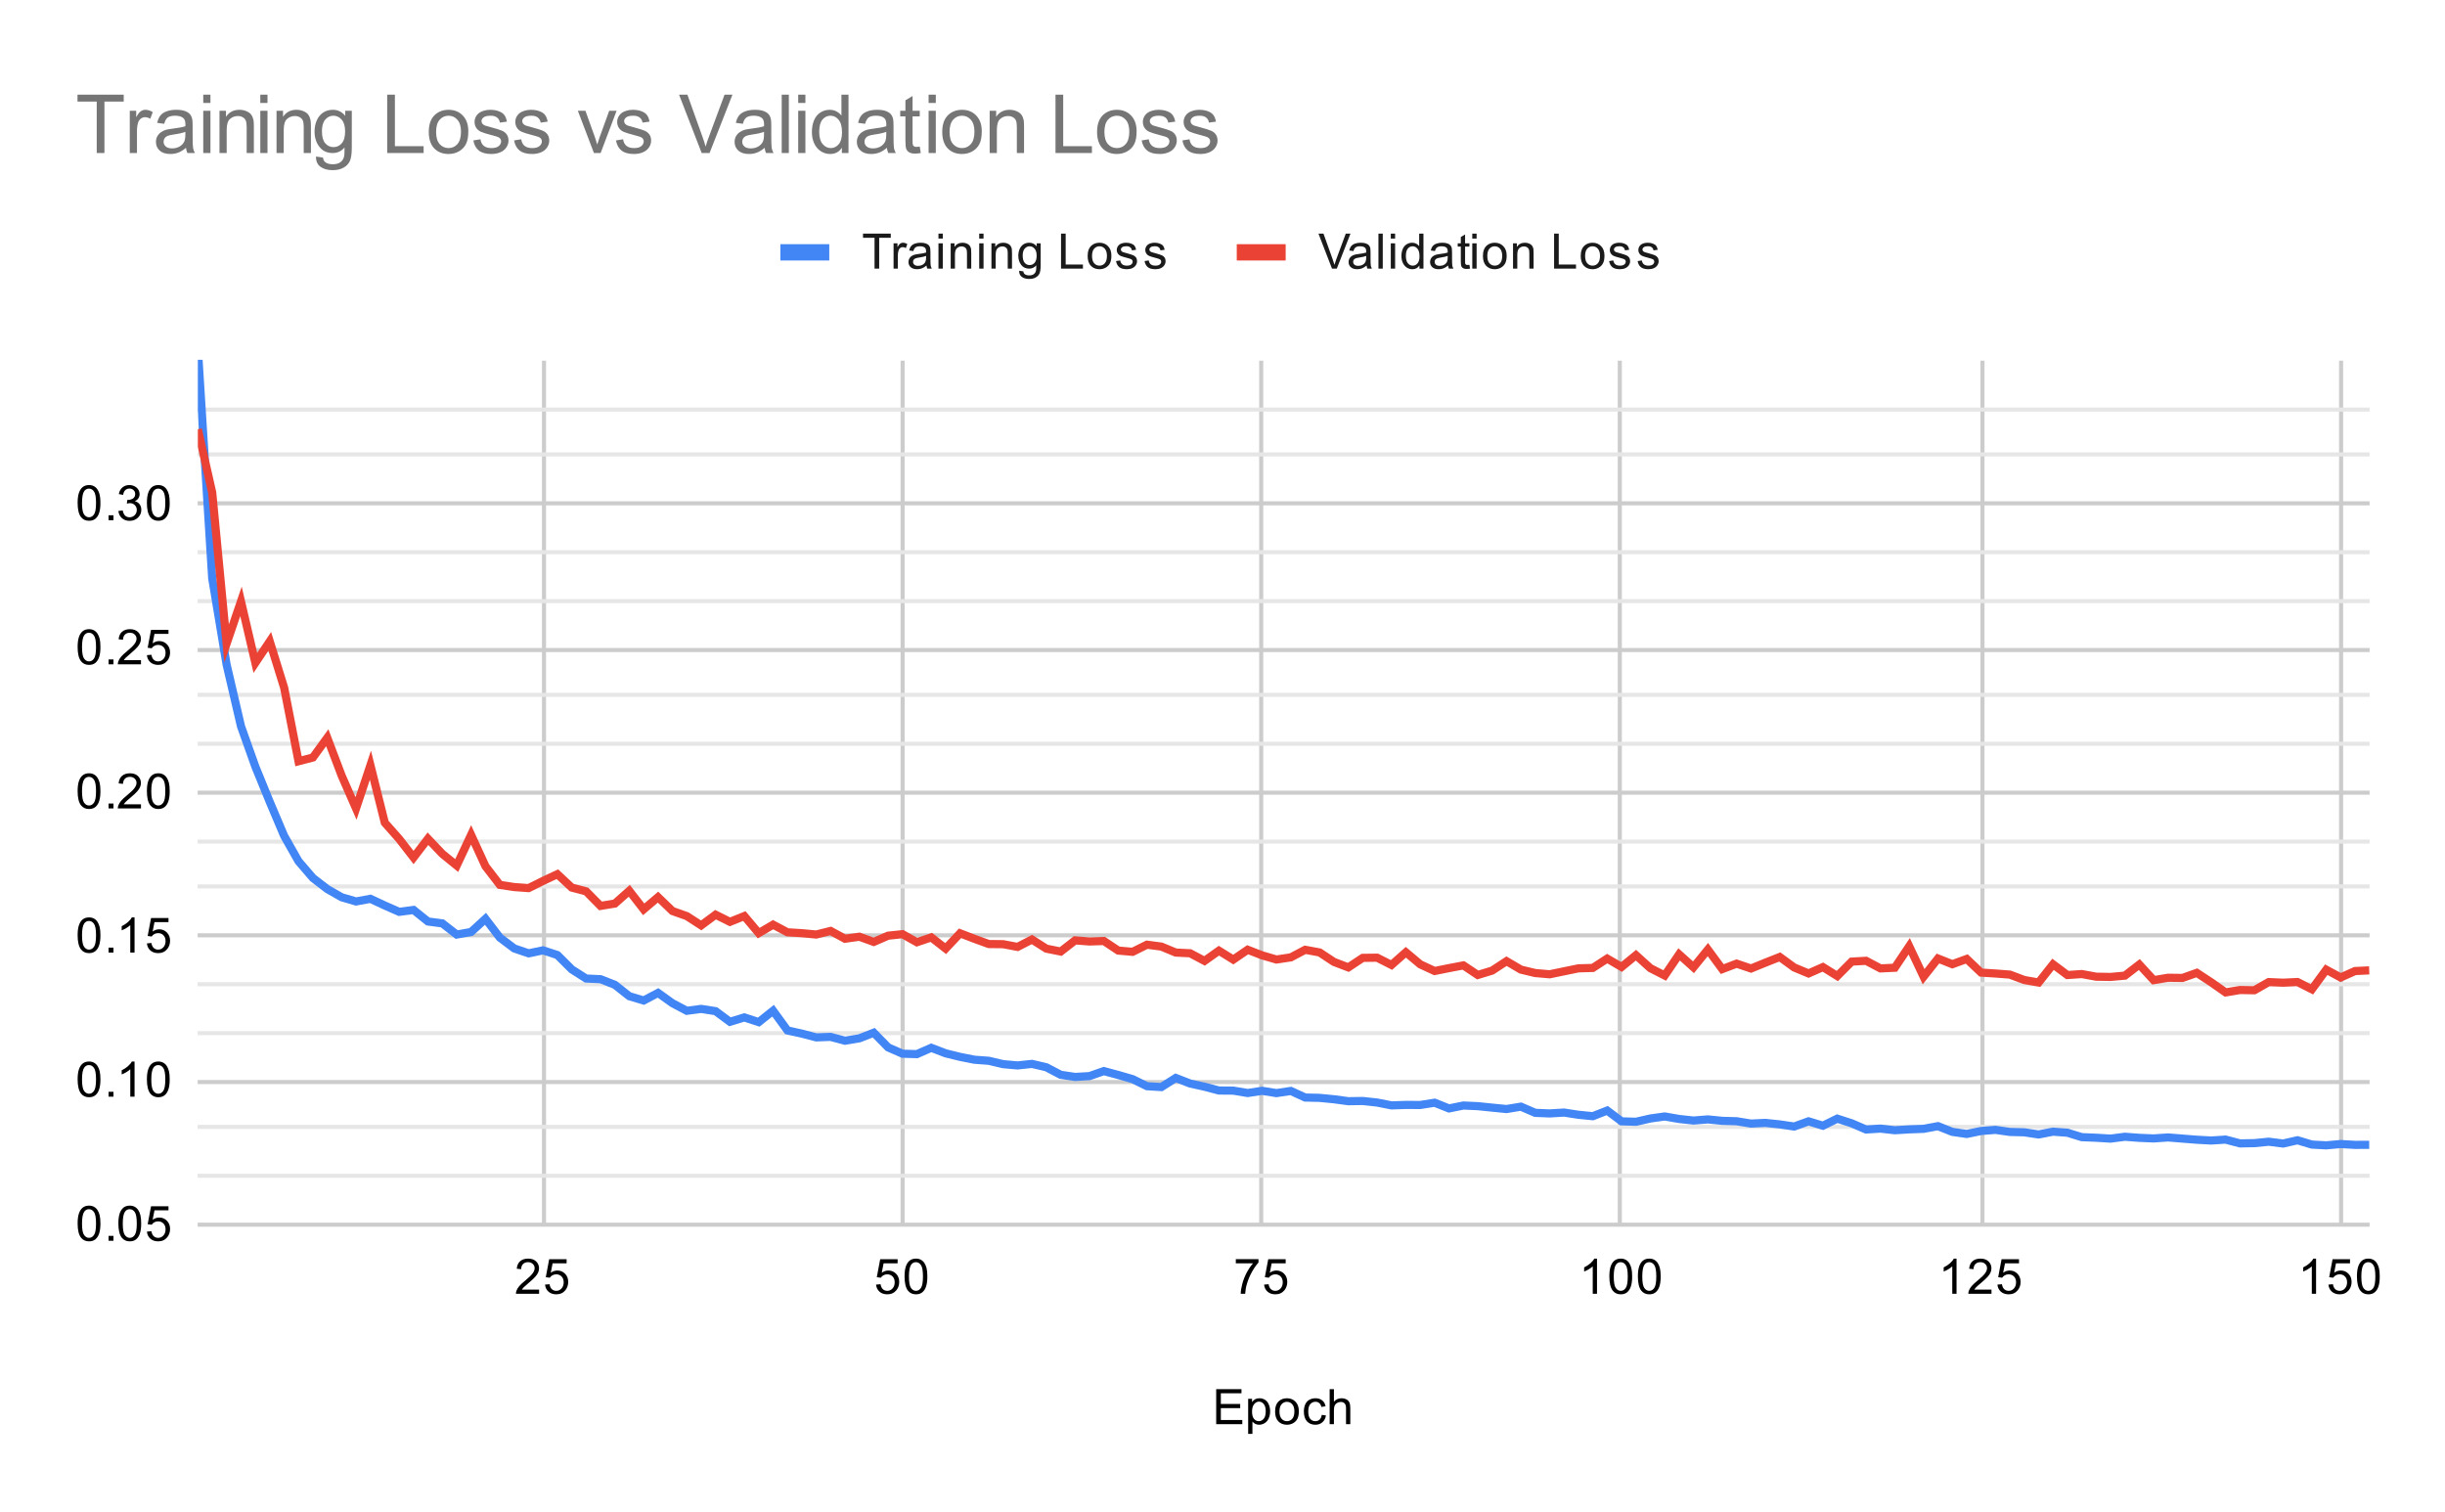
\includegraphics[width=0.3\textwidth]{figs/Project Charts/Training Loss vs Validation Loss.jpg} &
    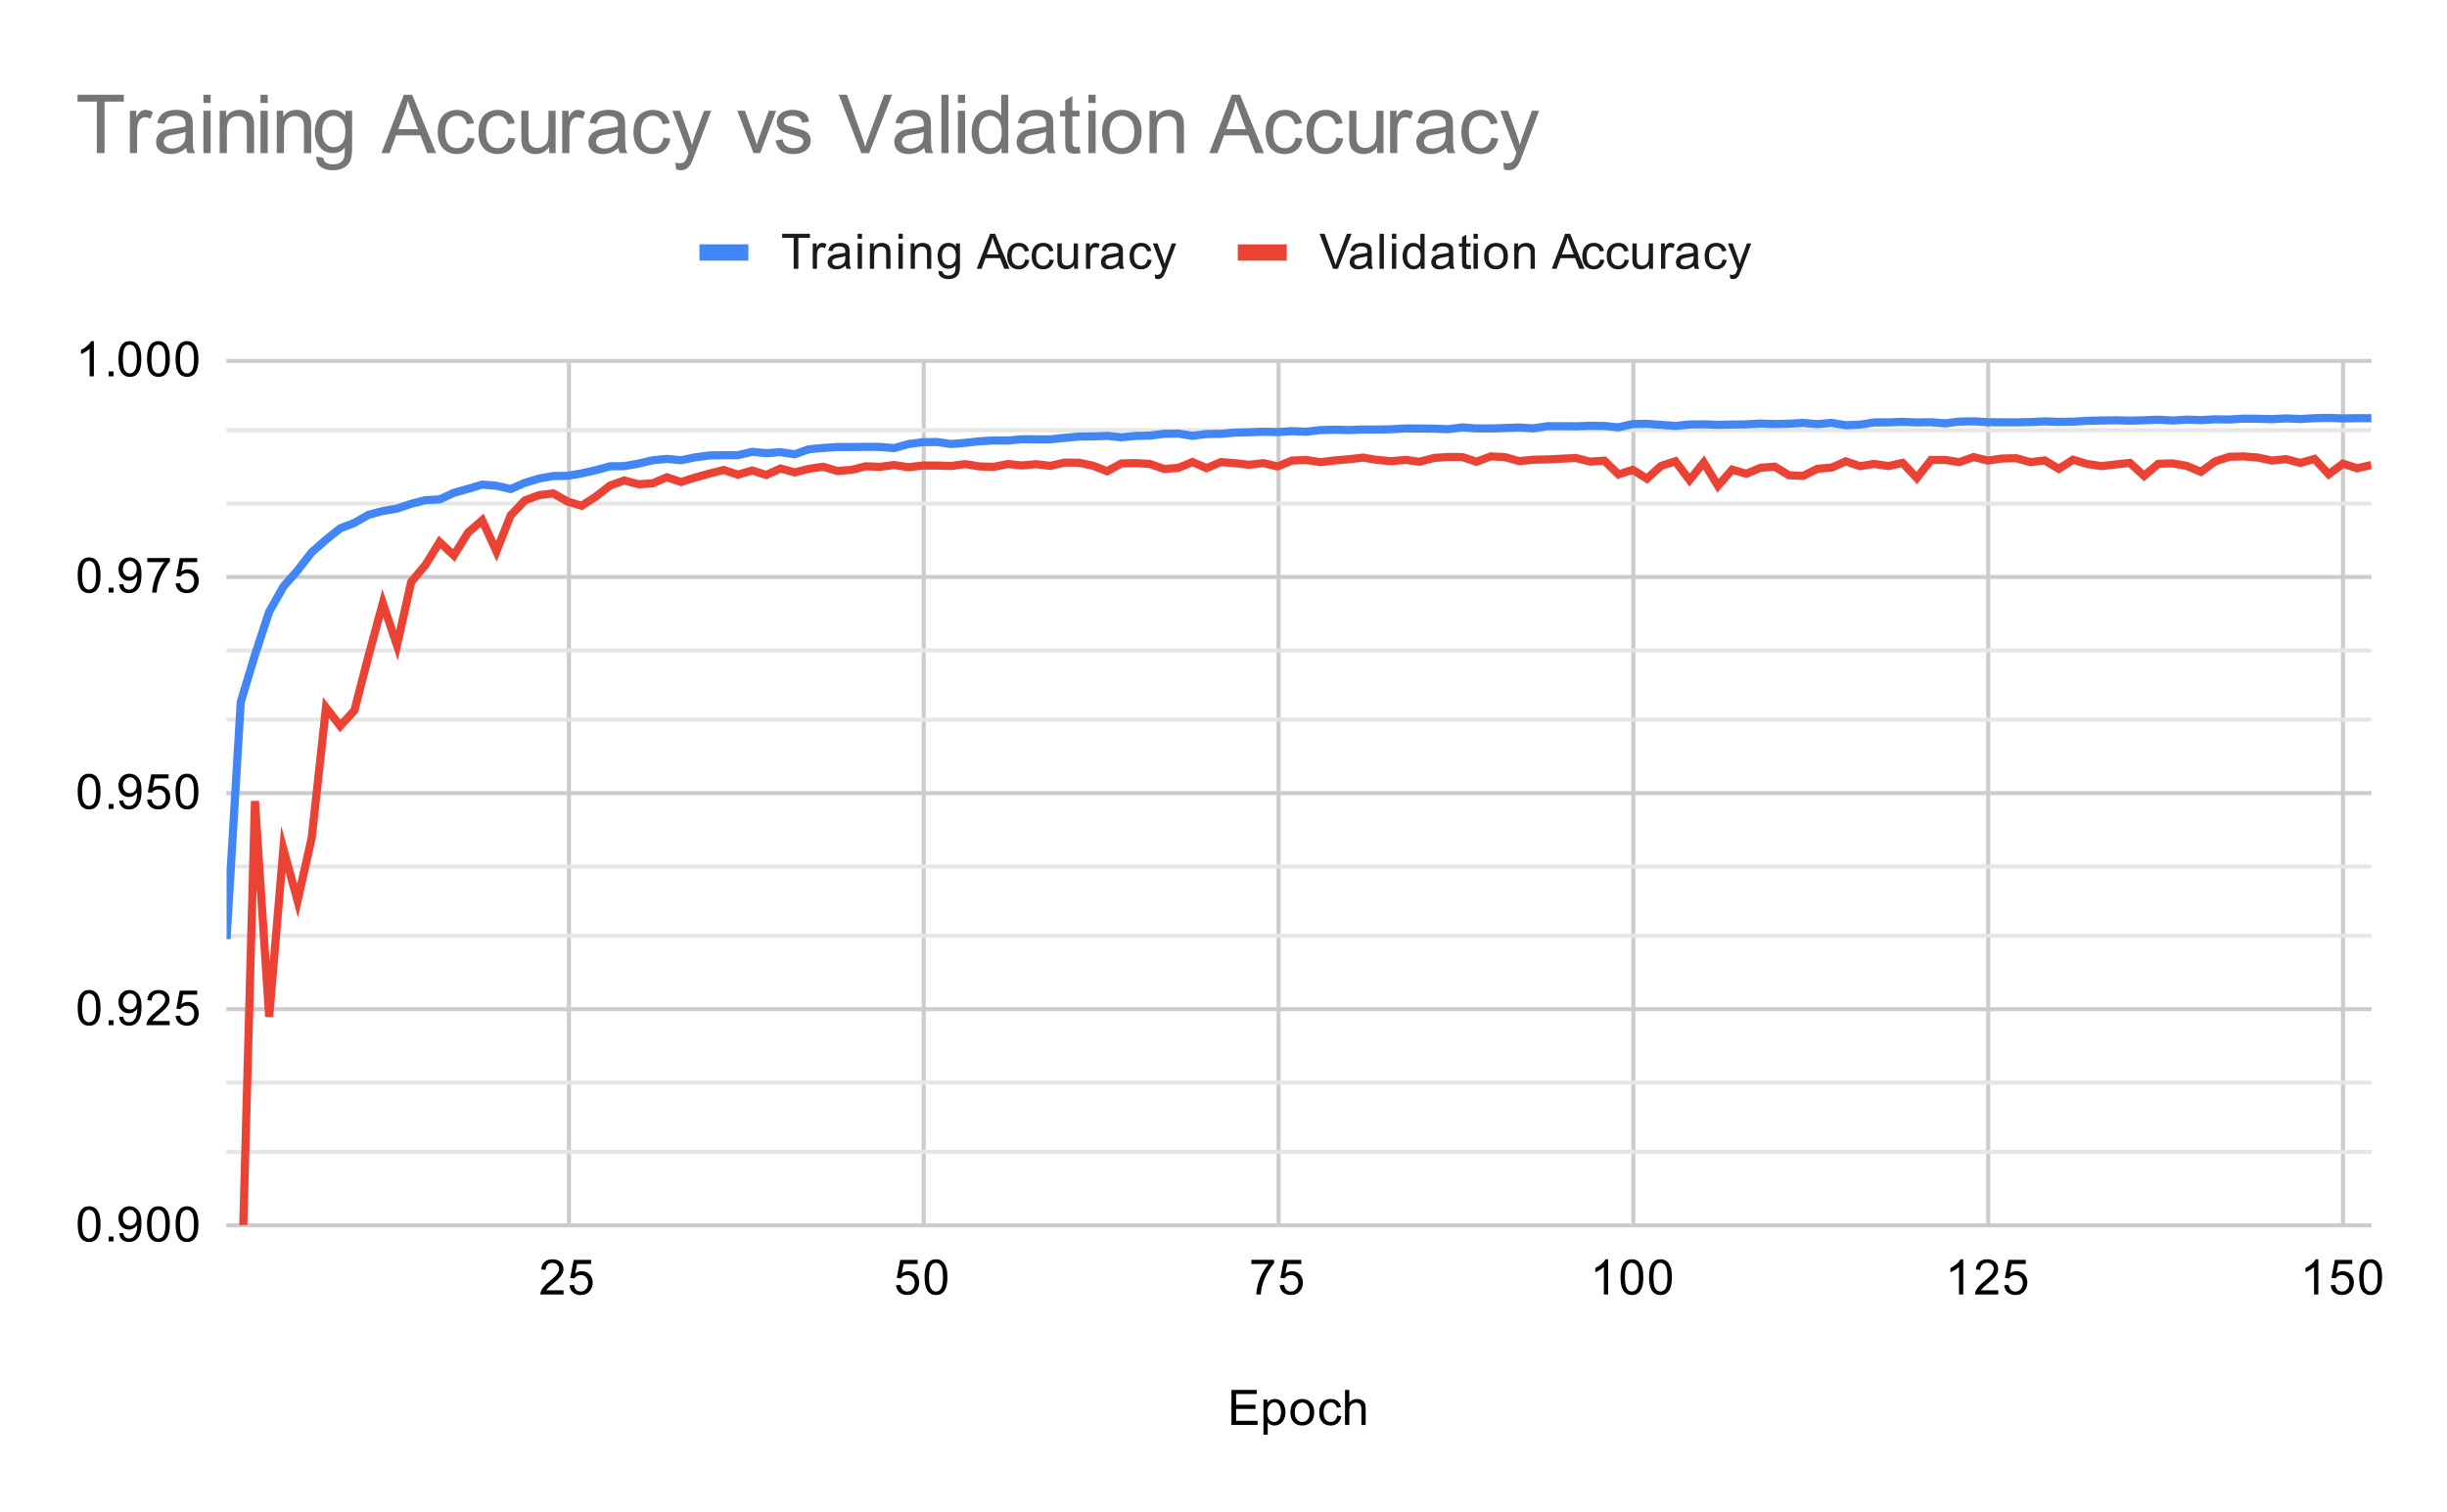
\includegraphics[width=0.3\textwidth]{figs/Project Charts/Training Accuracy vs Validation Accuracy.jpg} &
    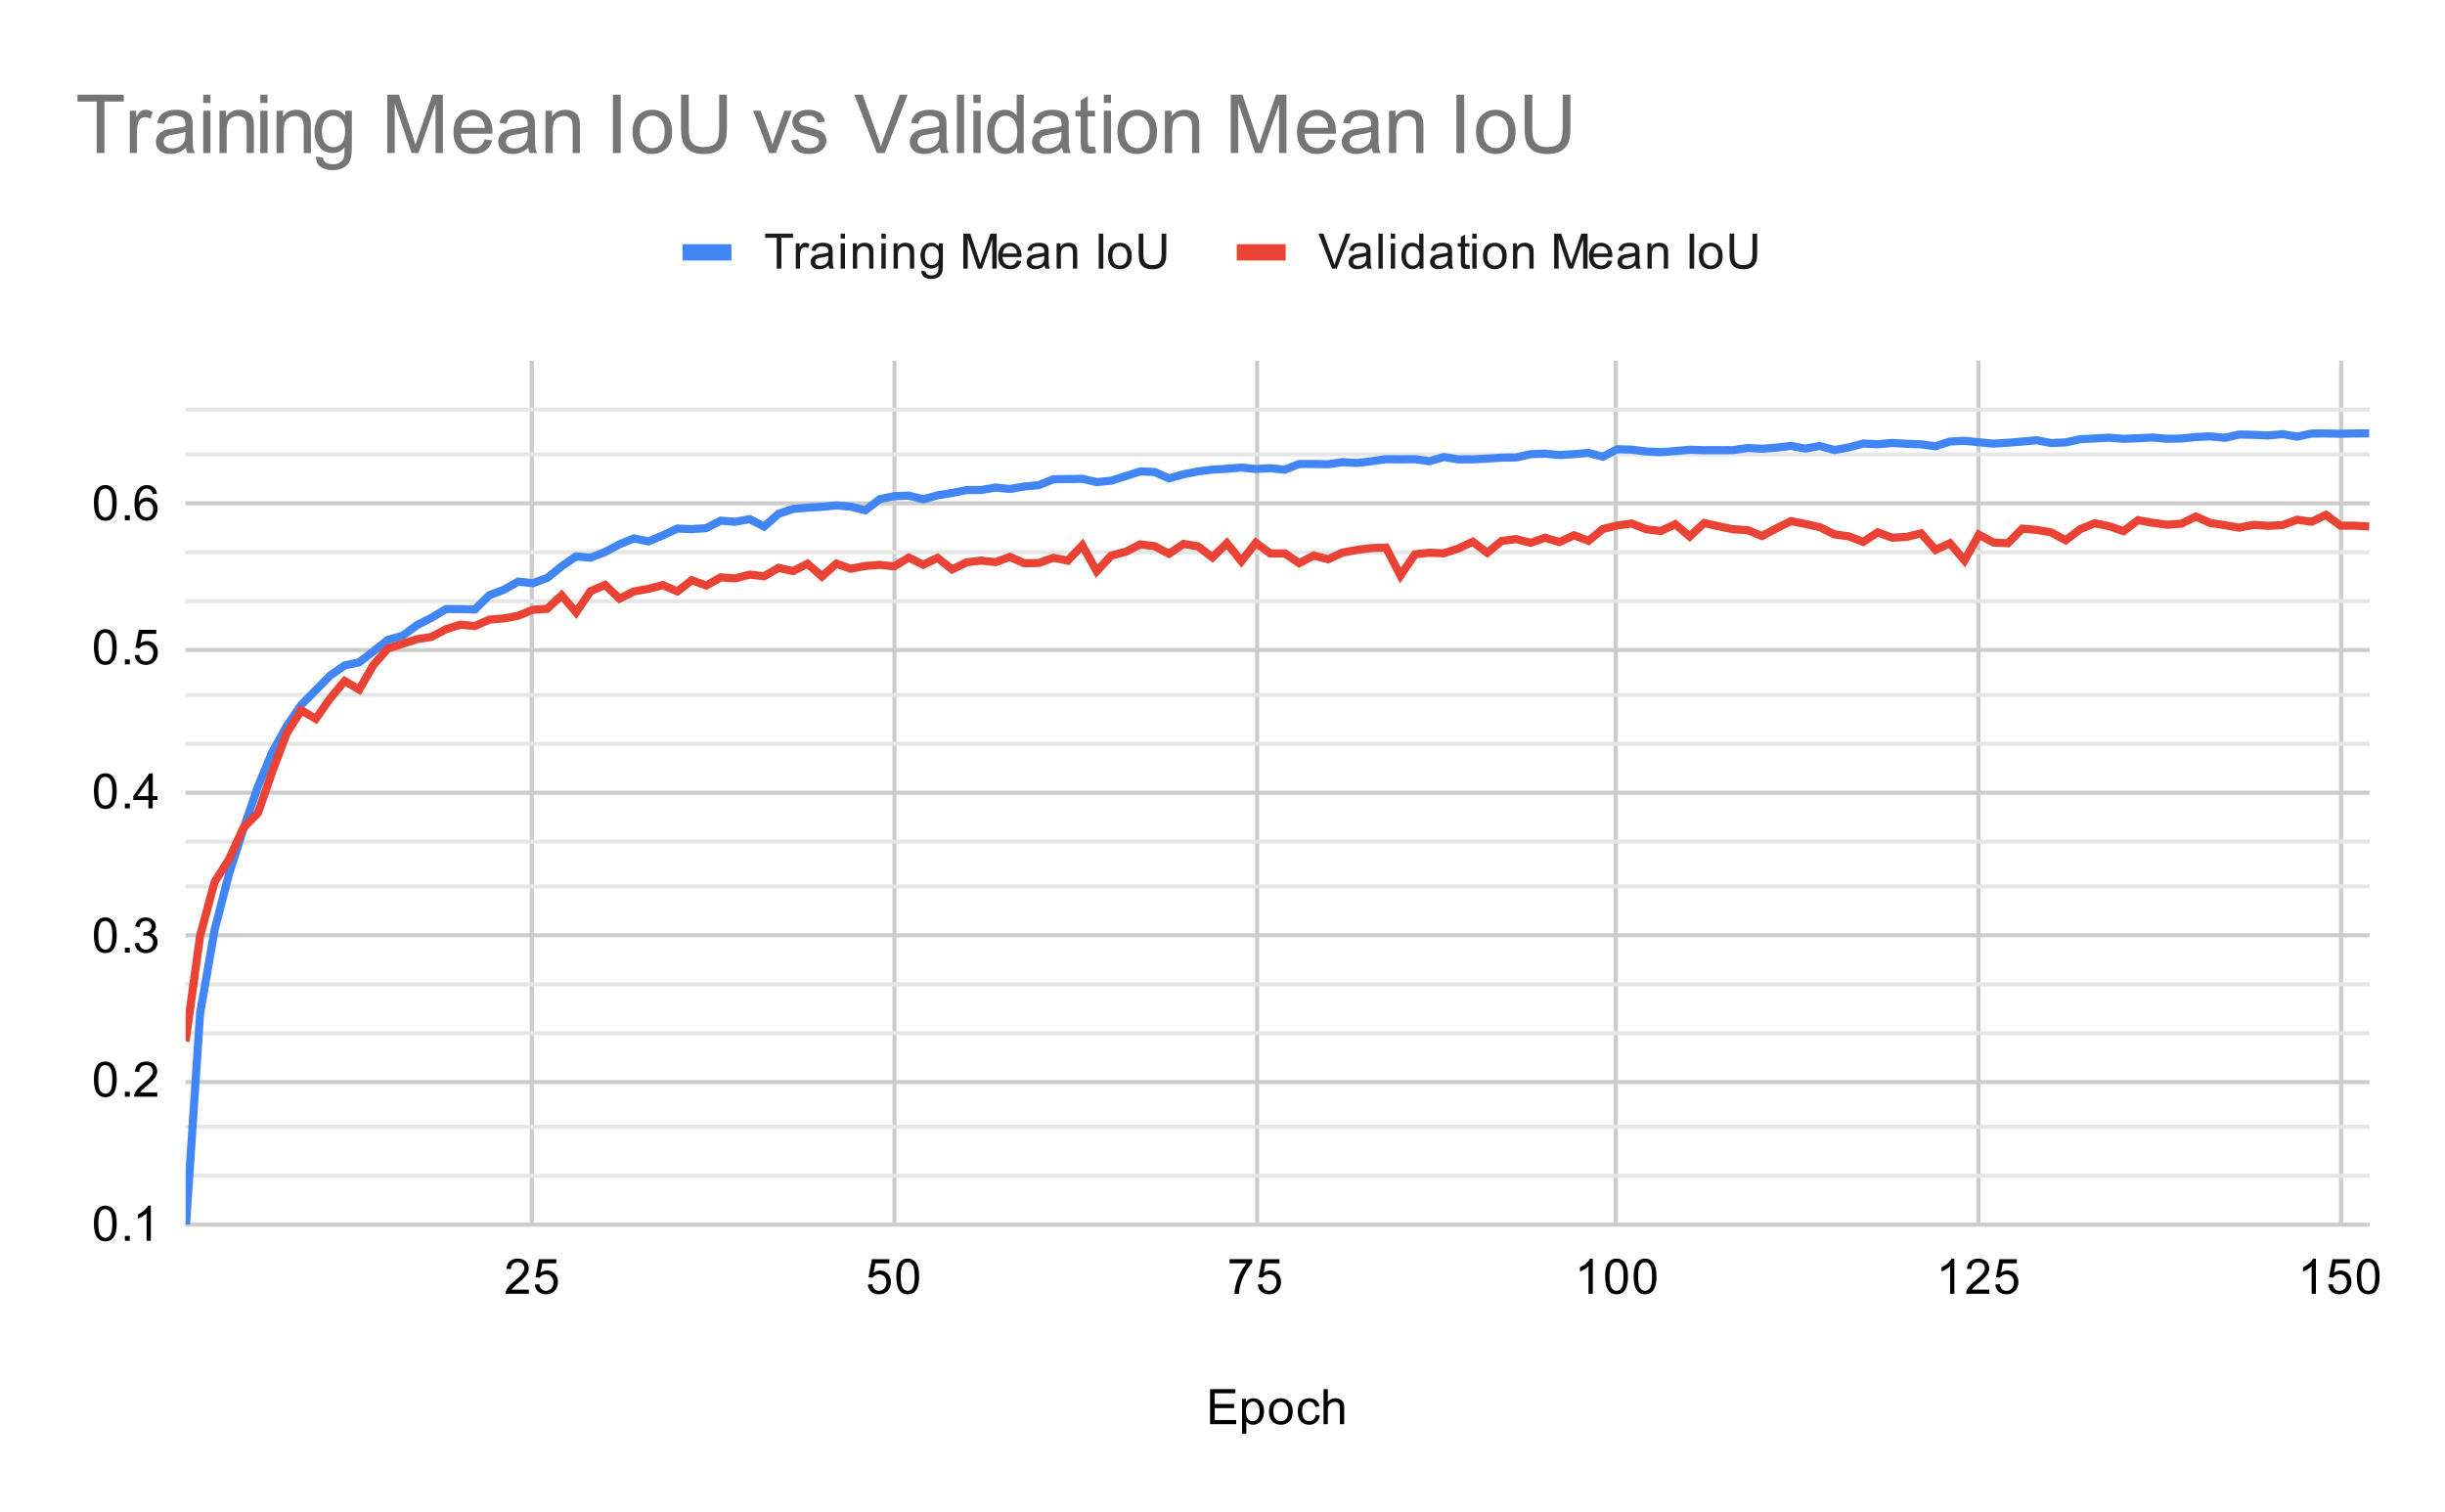
\includegraphics[width=0.3\textwidth]{figs/Project Charts/Training Mean IoU vs Validation Mean IoU.jpg} \\

    (a) Loss Graph & (b) Accuracy Graph & (c) Mean IoU Graph \\[6pt]

    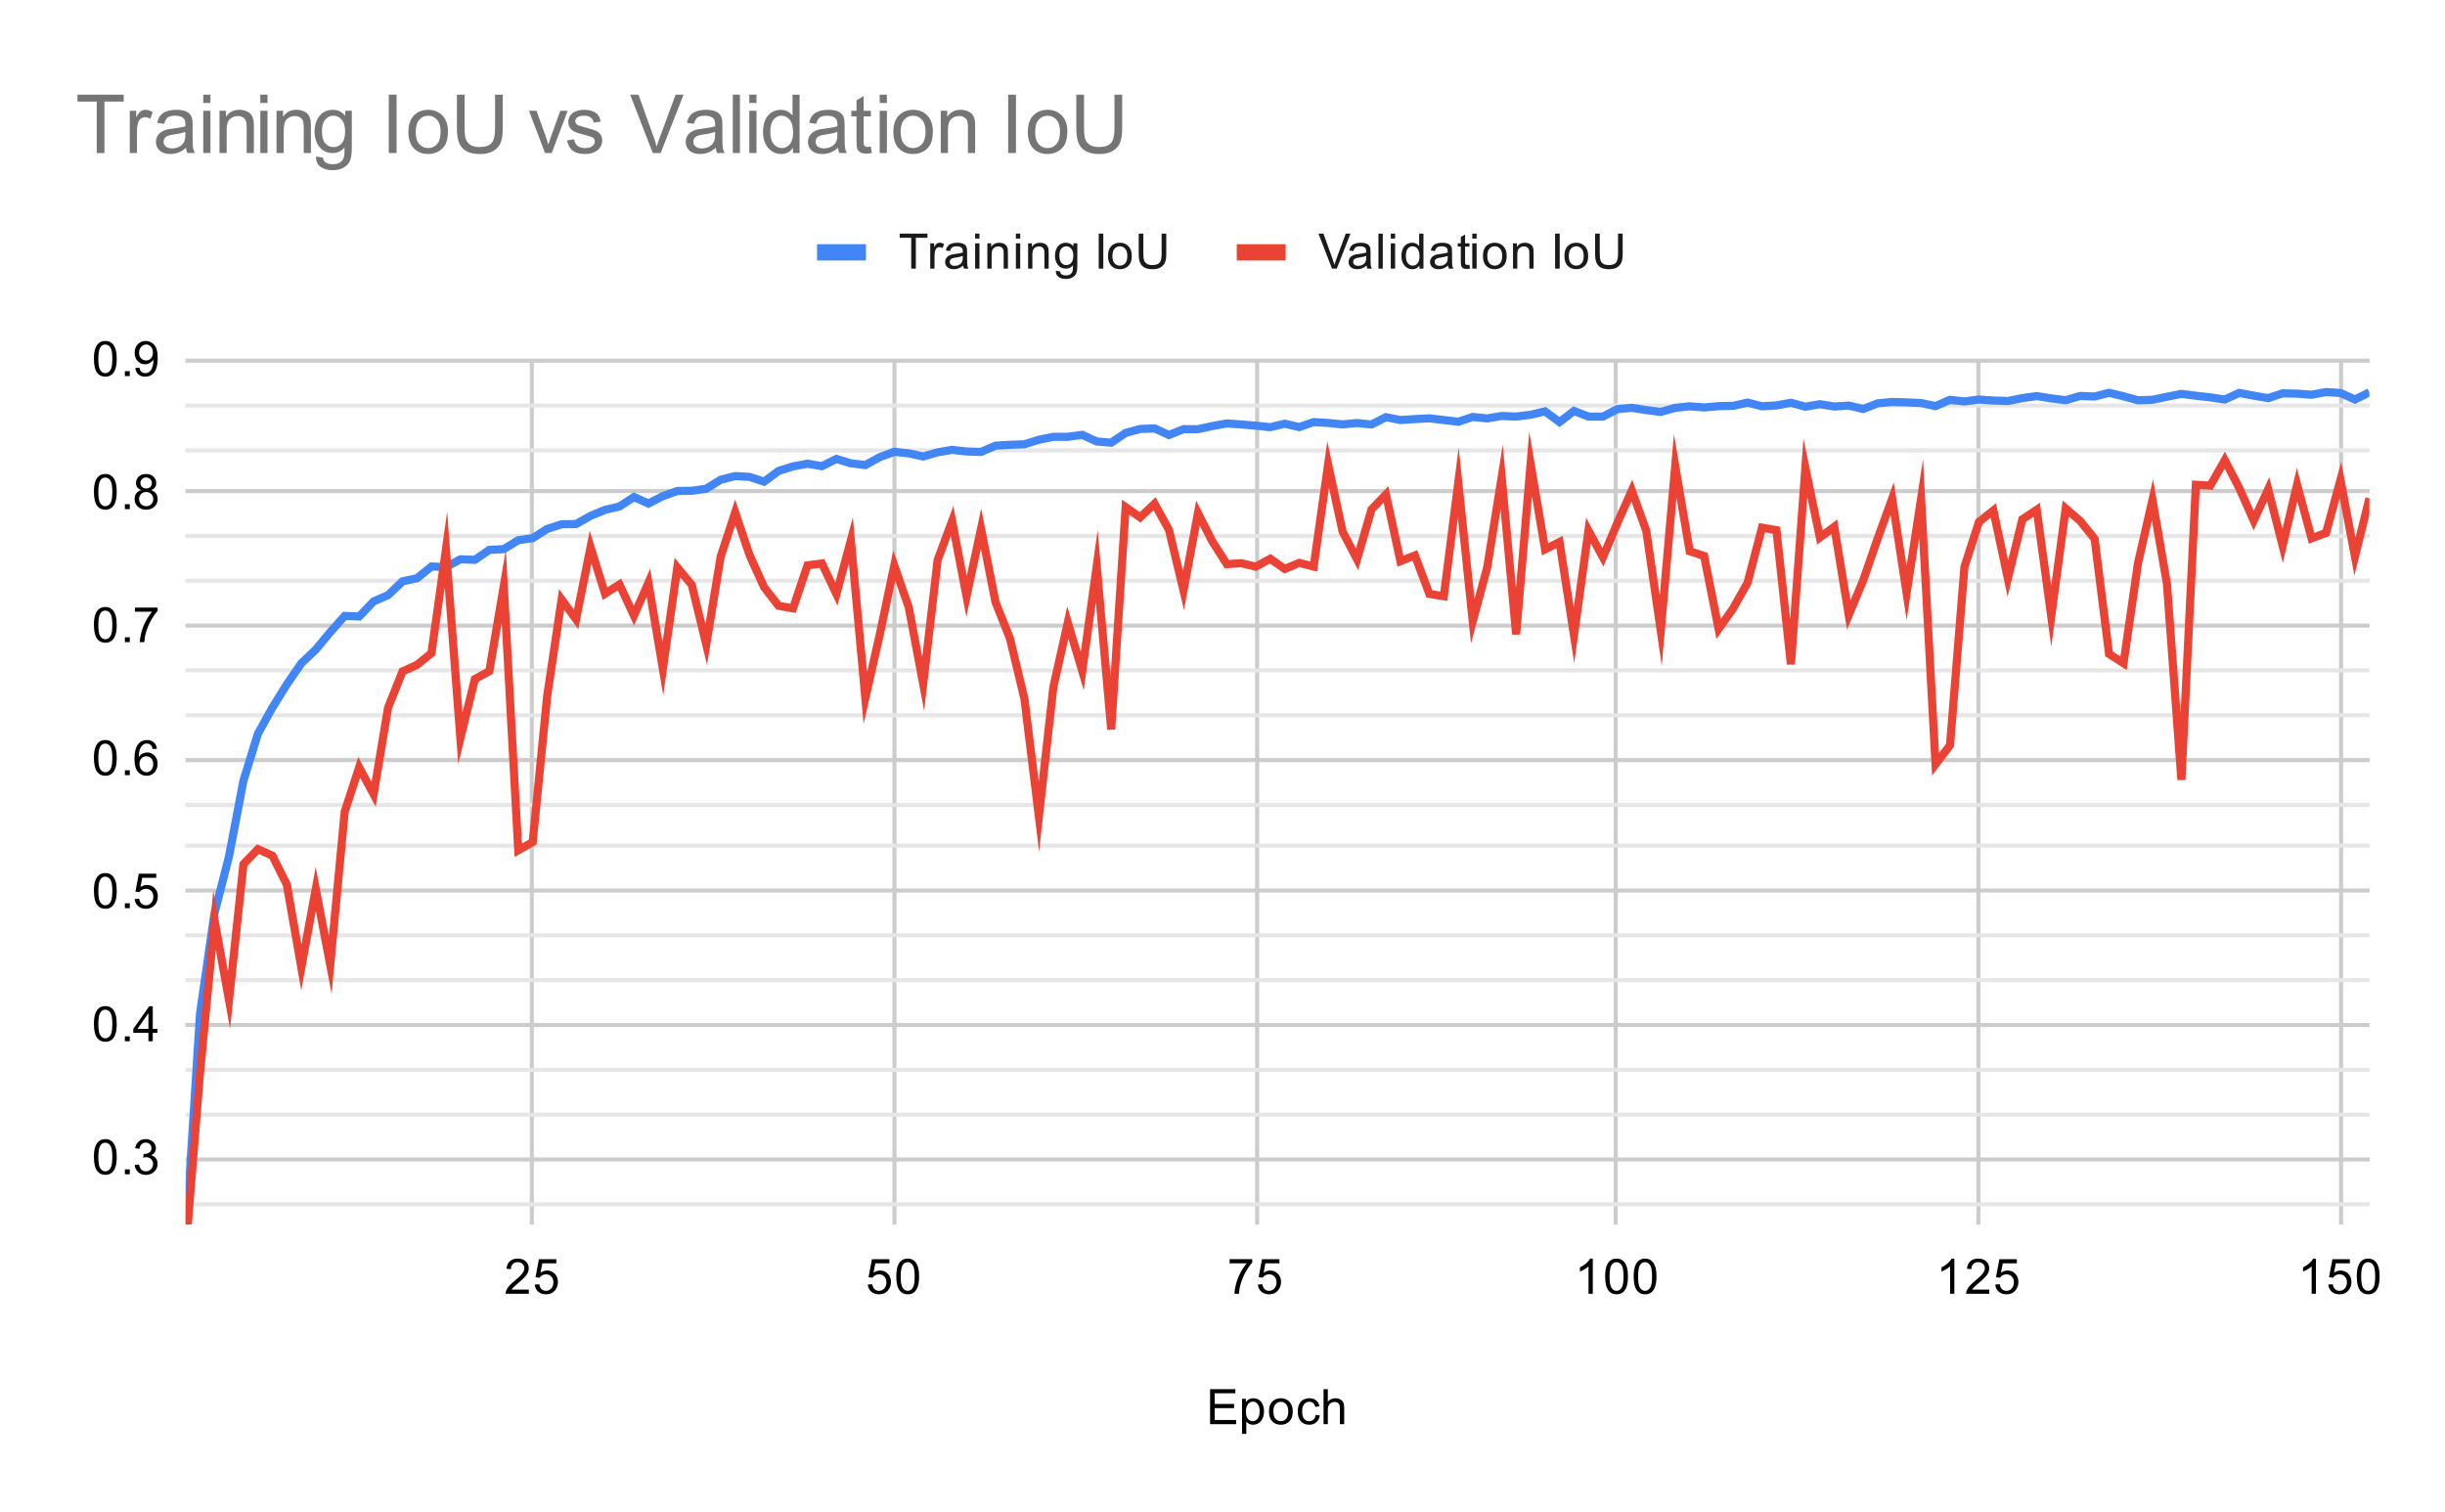
\includegraphics[width=0.3\textwidth]{figs/Project Charts/Training IoU vs Validation IoU.jpg} &
    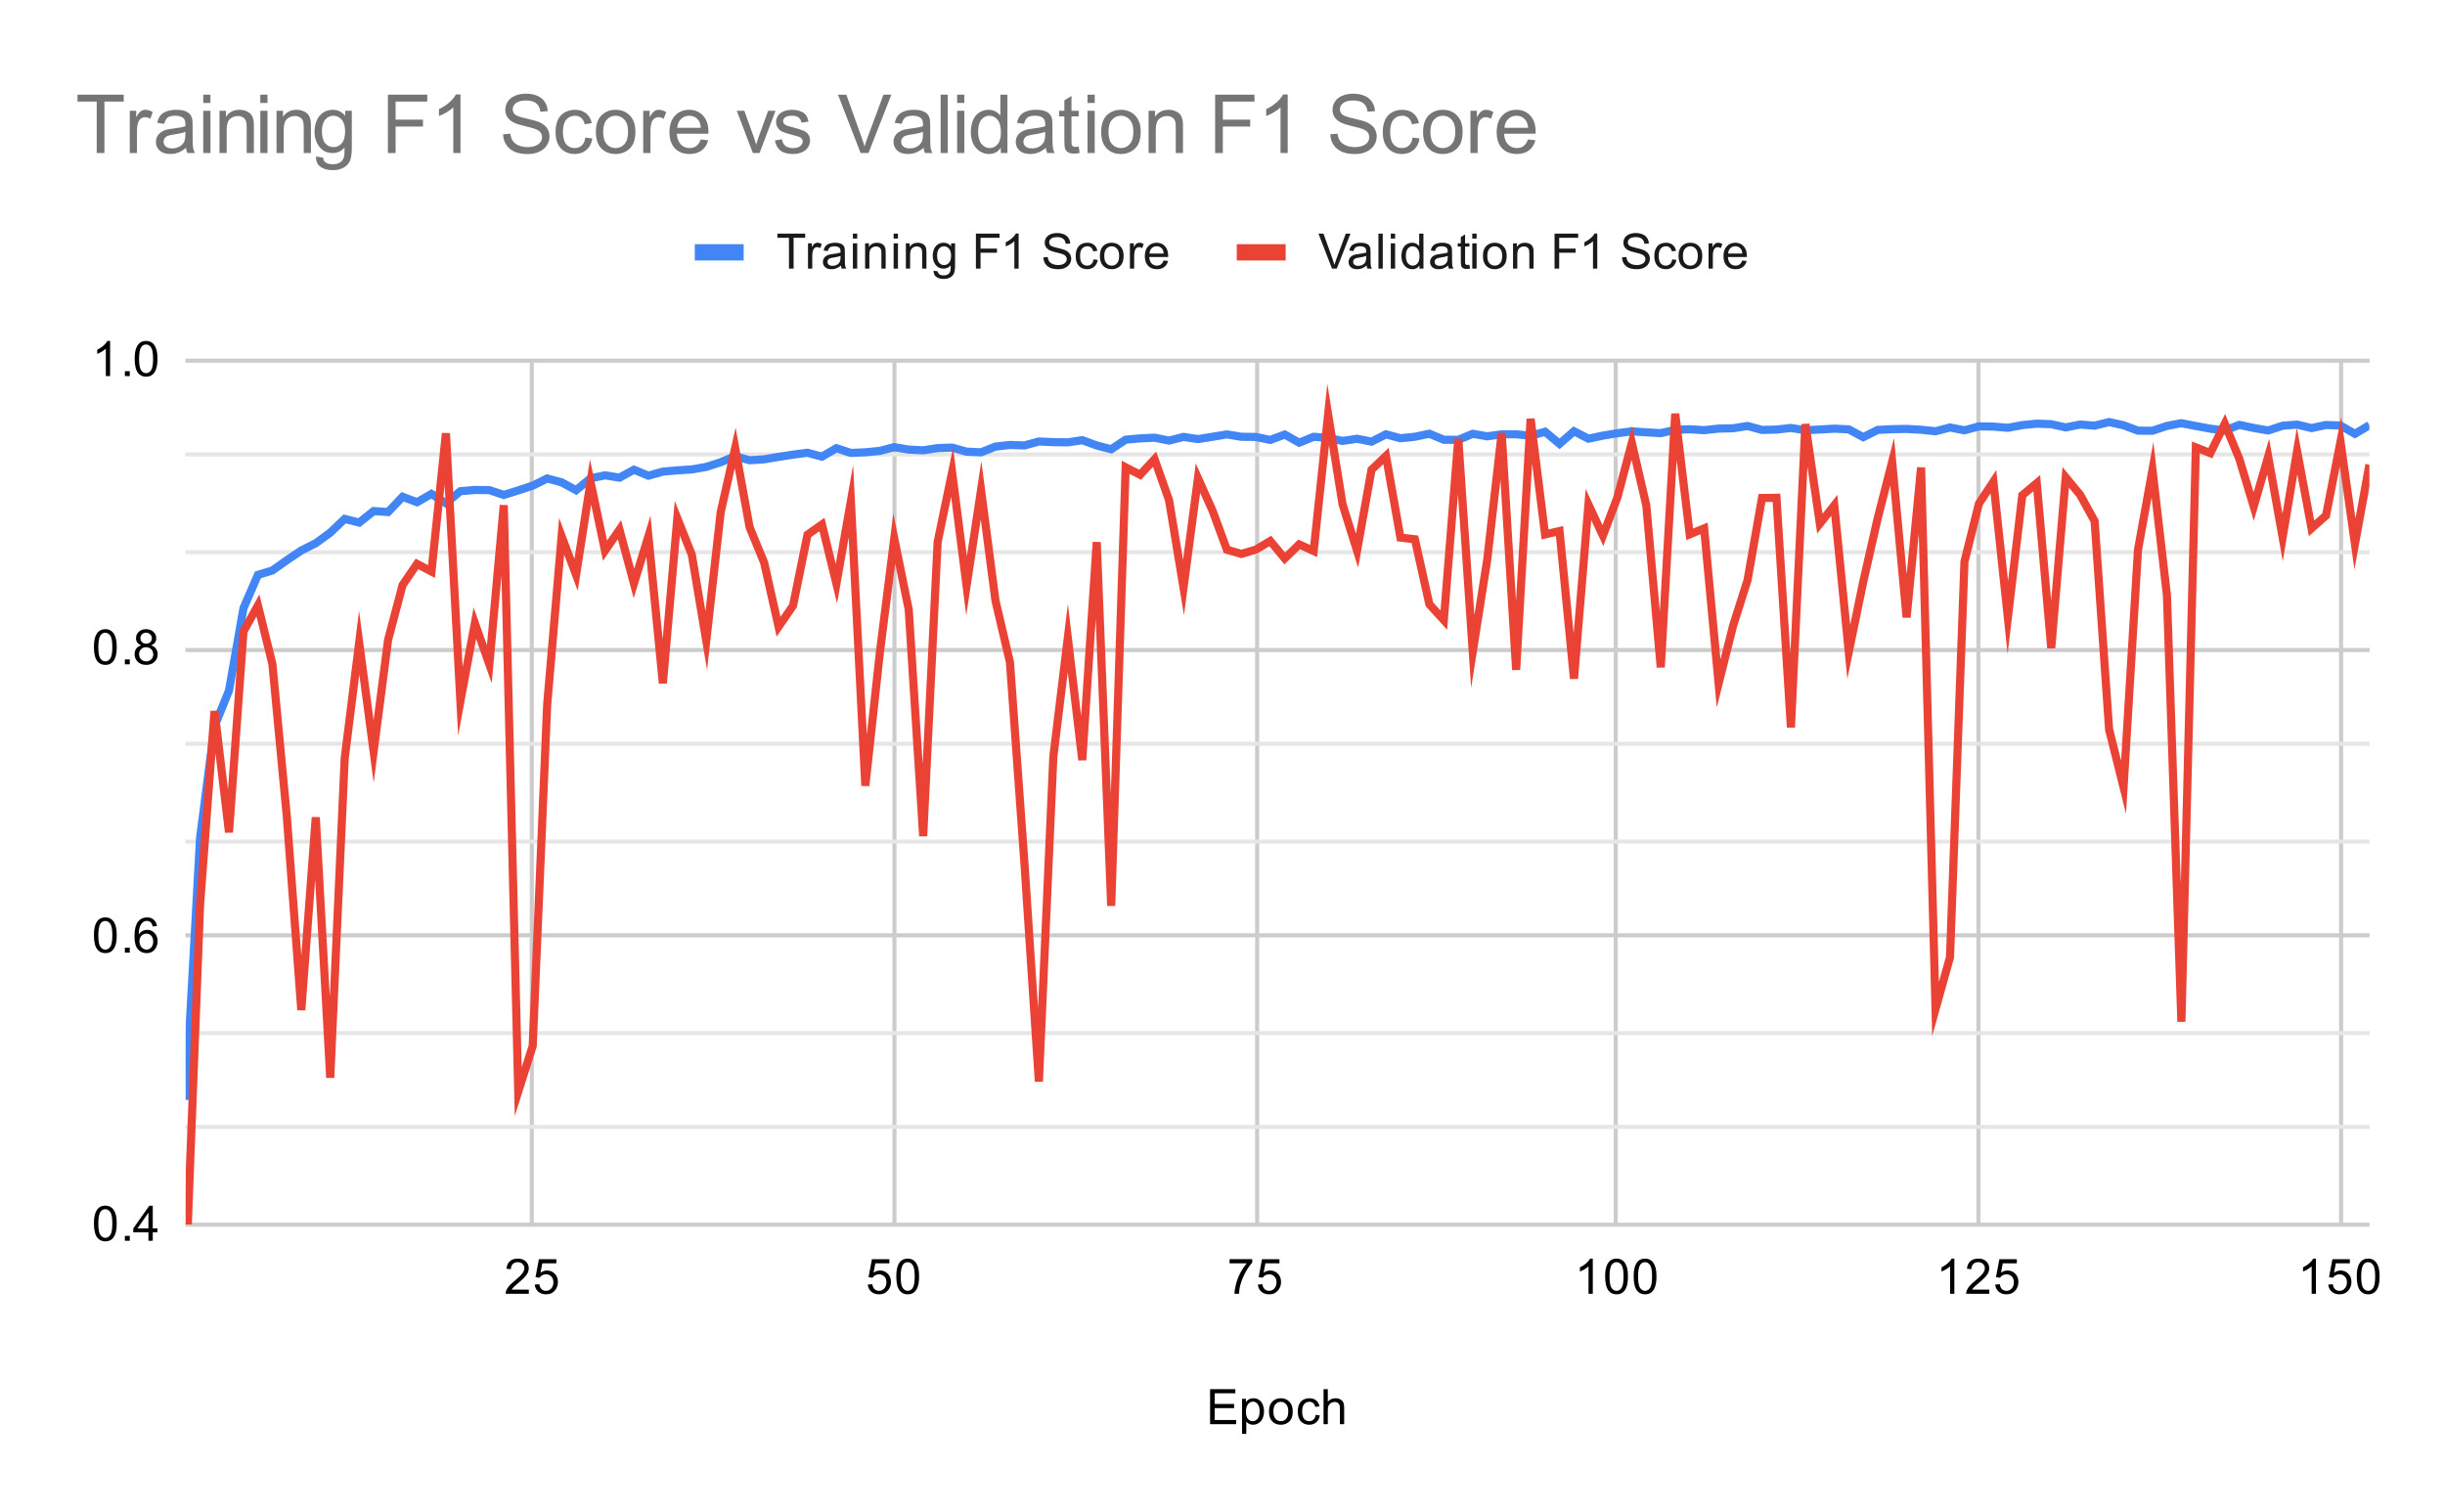
\includegraphics[width=0.3\textwidth]{figs/Project Charts/Training F1 Score vs Validation F1 Score.jpg} &
    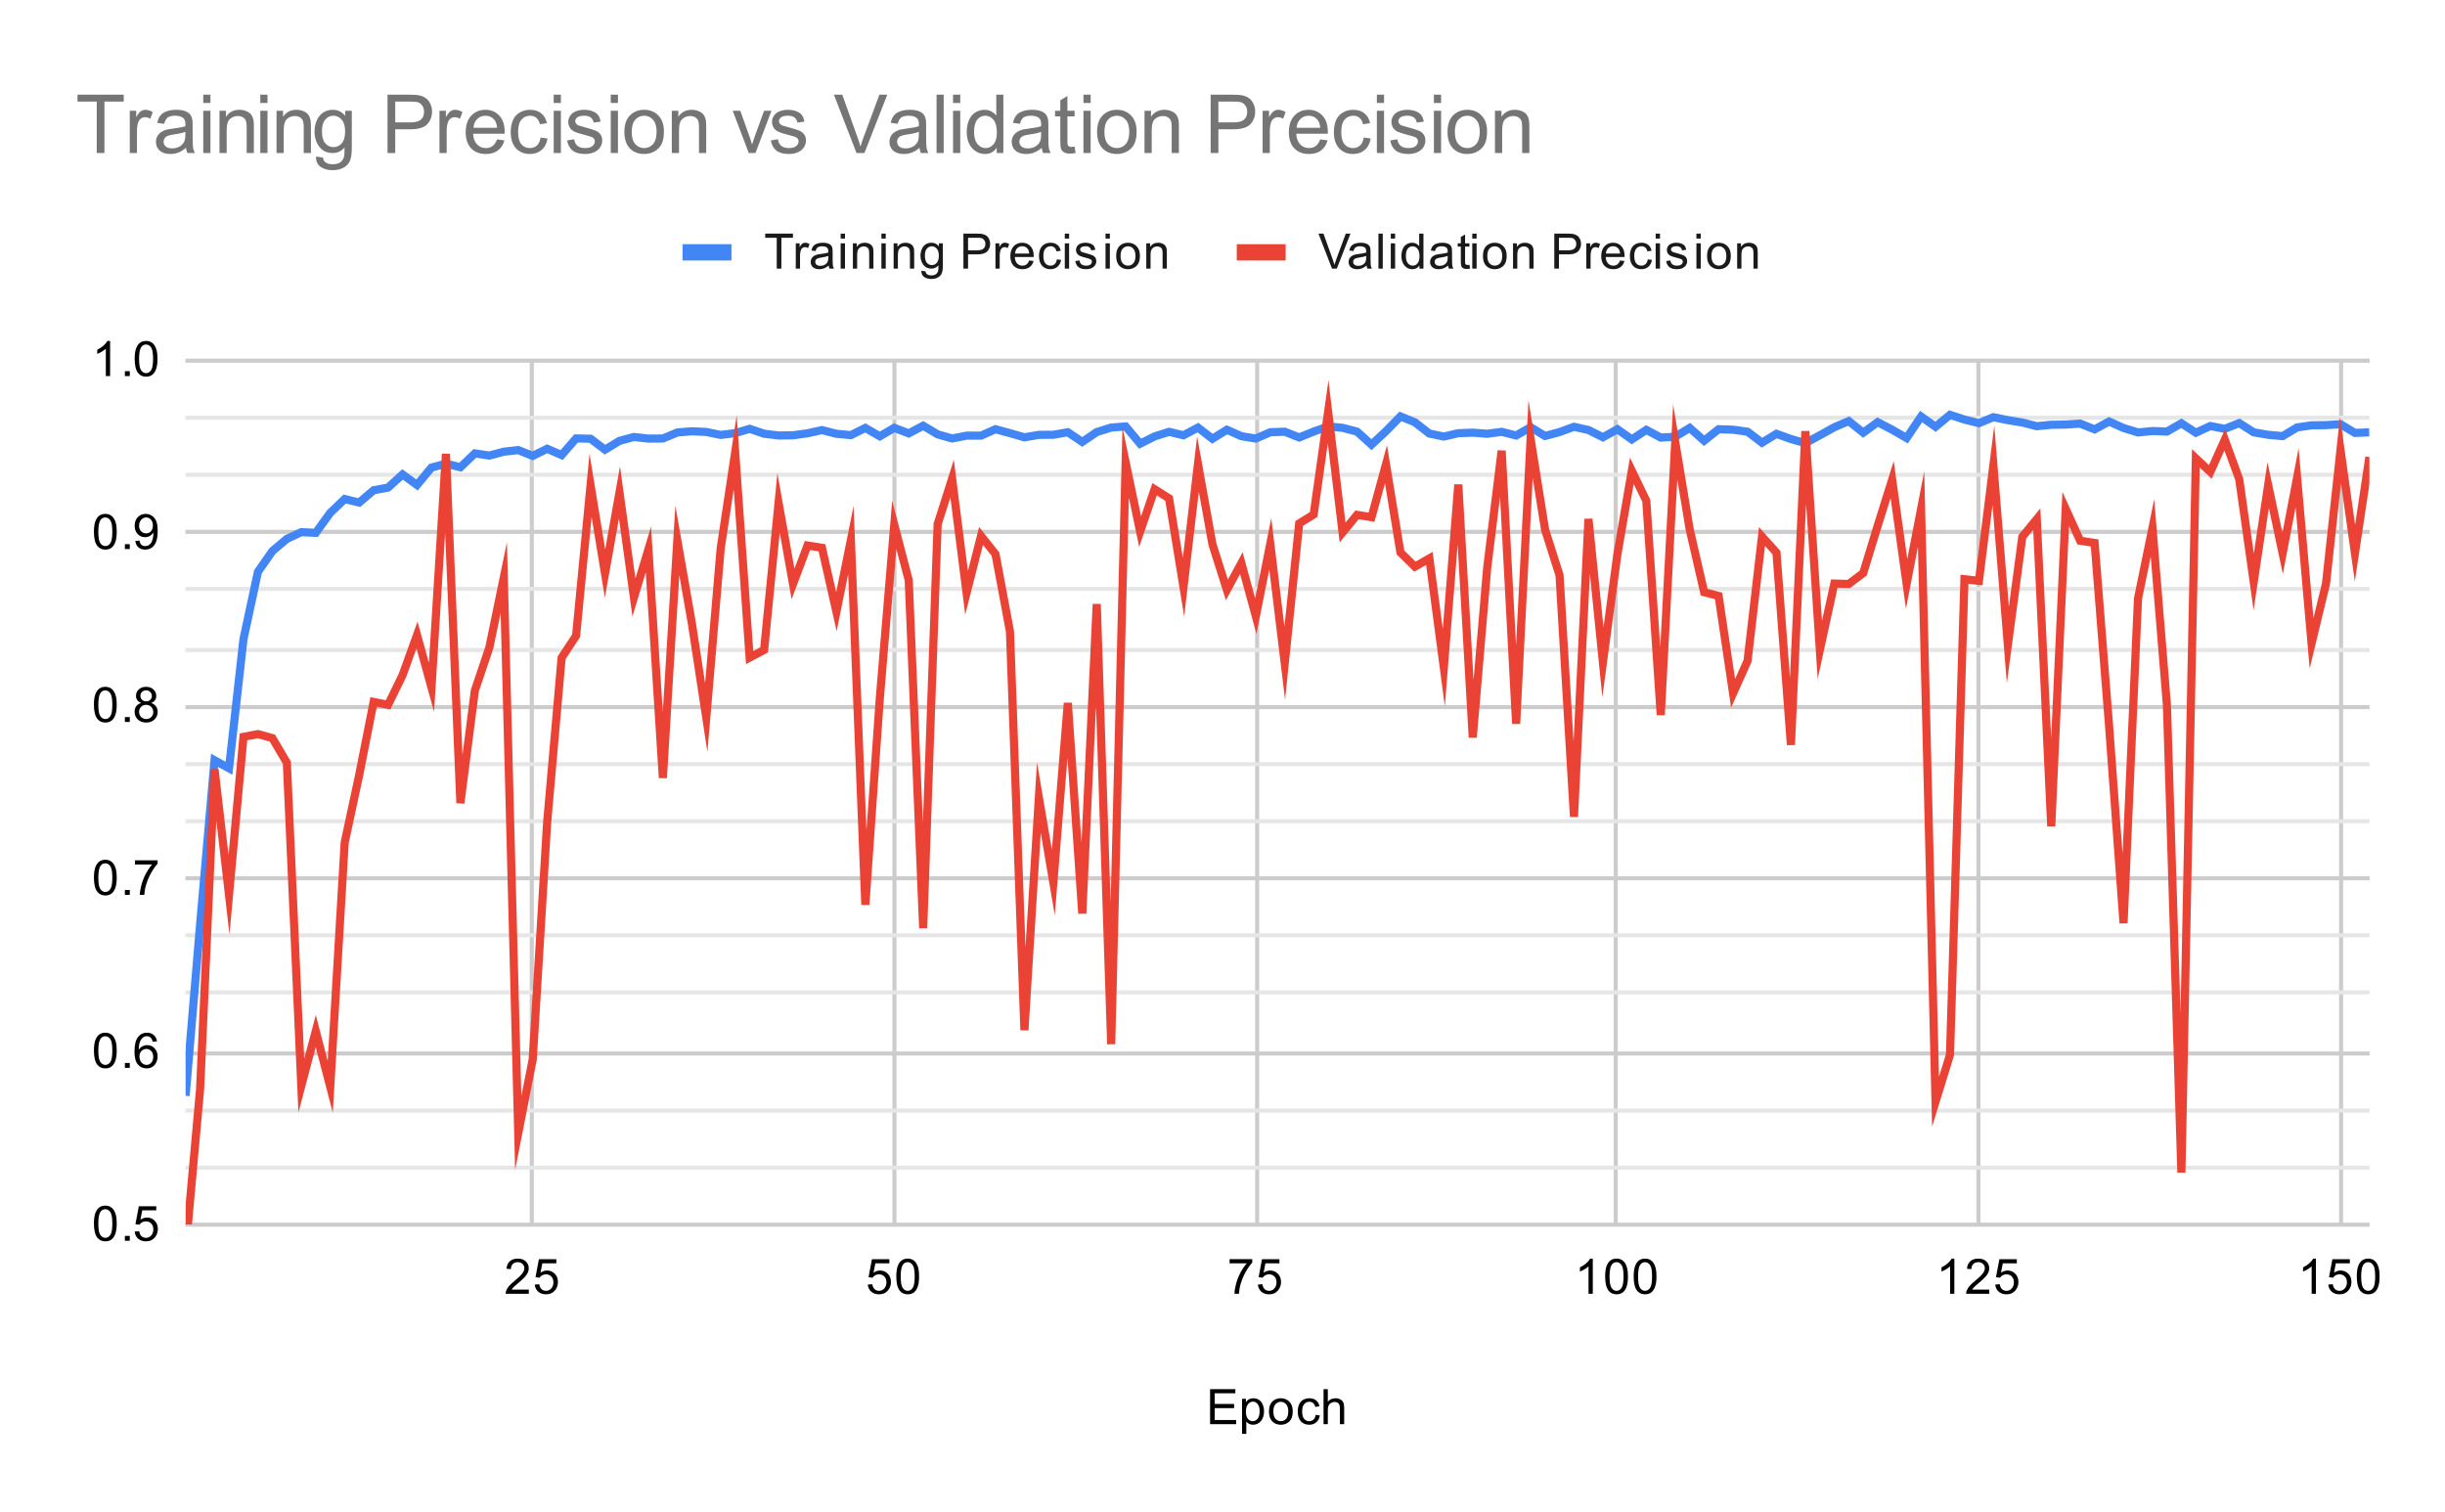
\includegraphics[width=0.3\textwidth]{figs/Project Charts/Training Precision vs Validation Precision.jpg} \\

    (d) IoU Graph & (e) F1 Score Graph & (f) Precision Graph \\[6pt]

    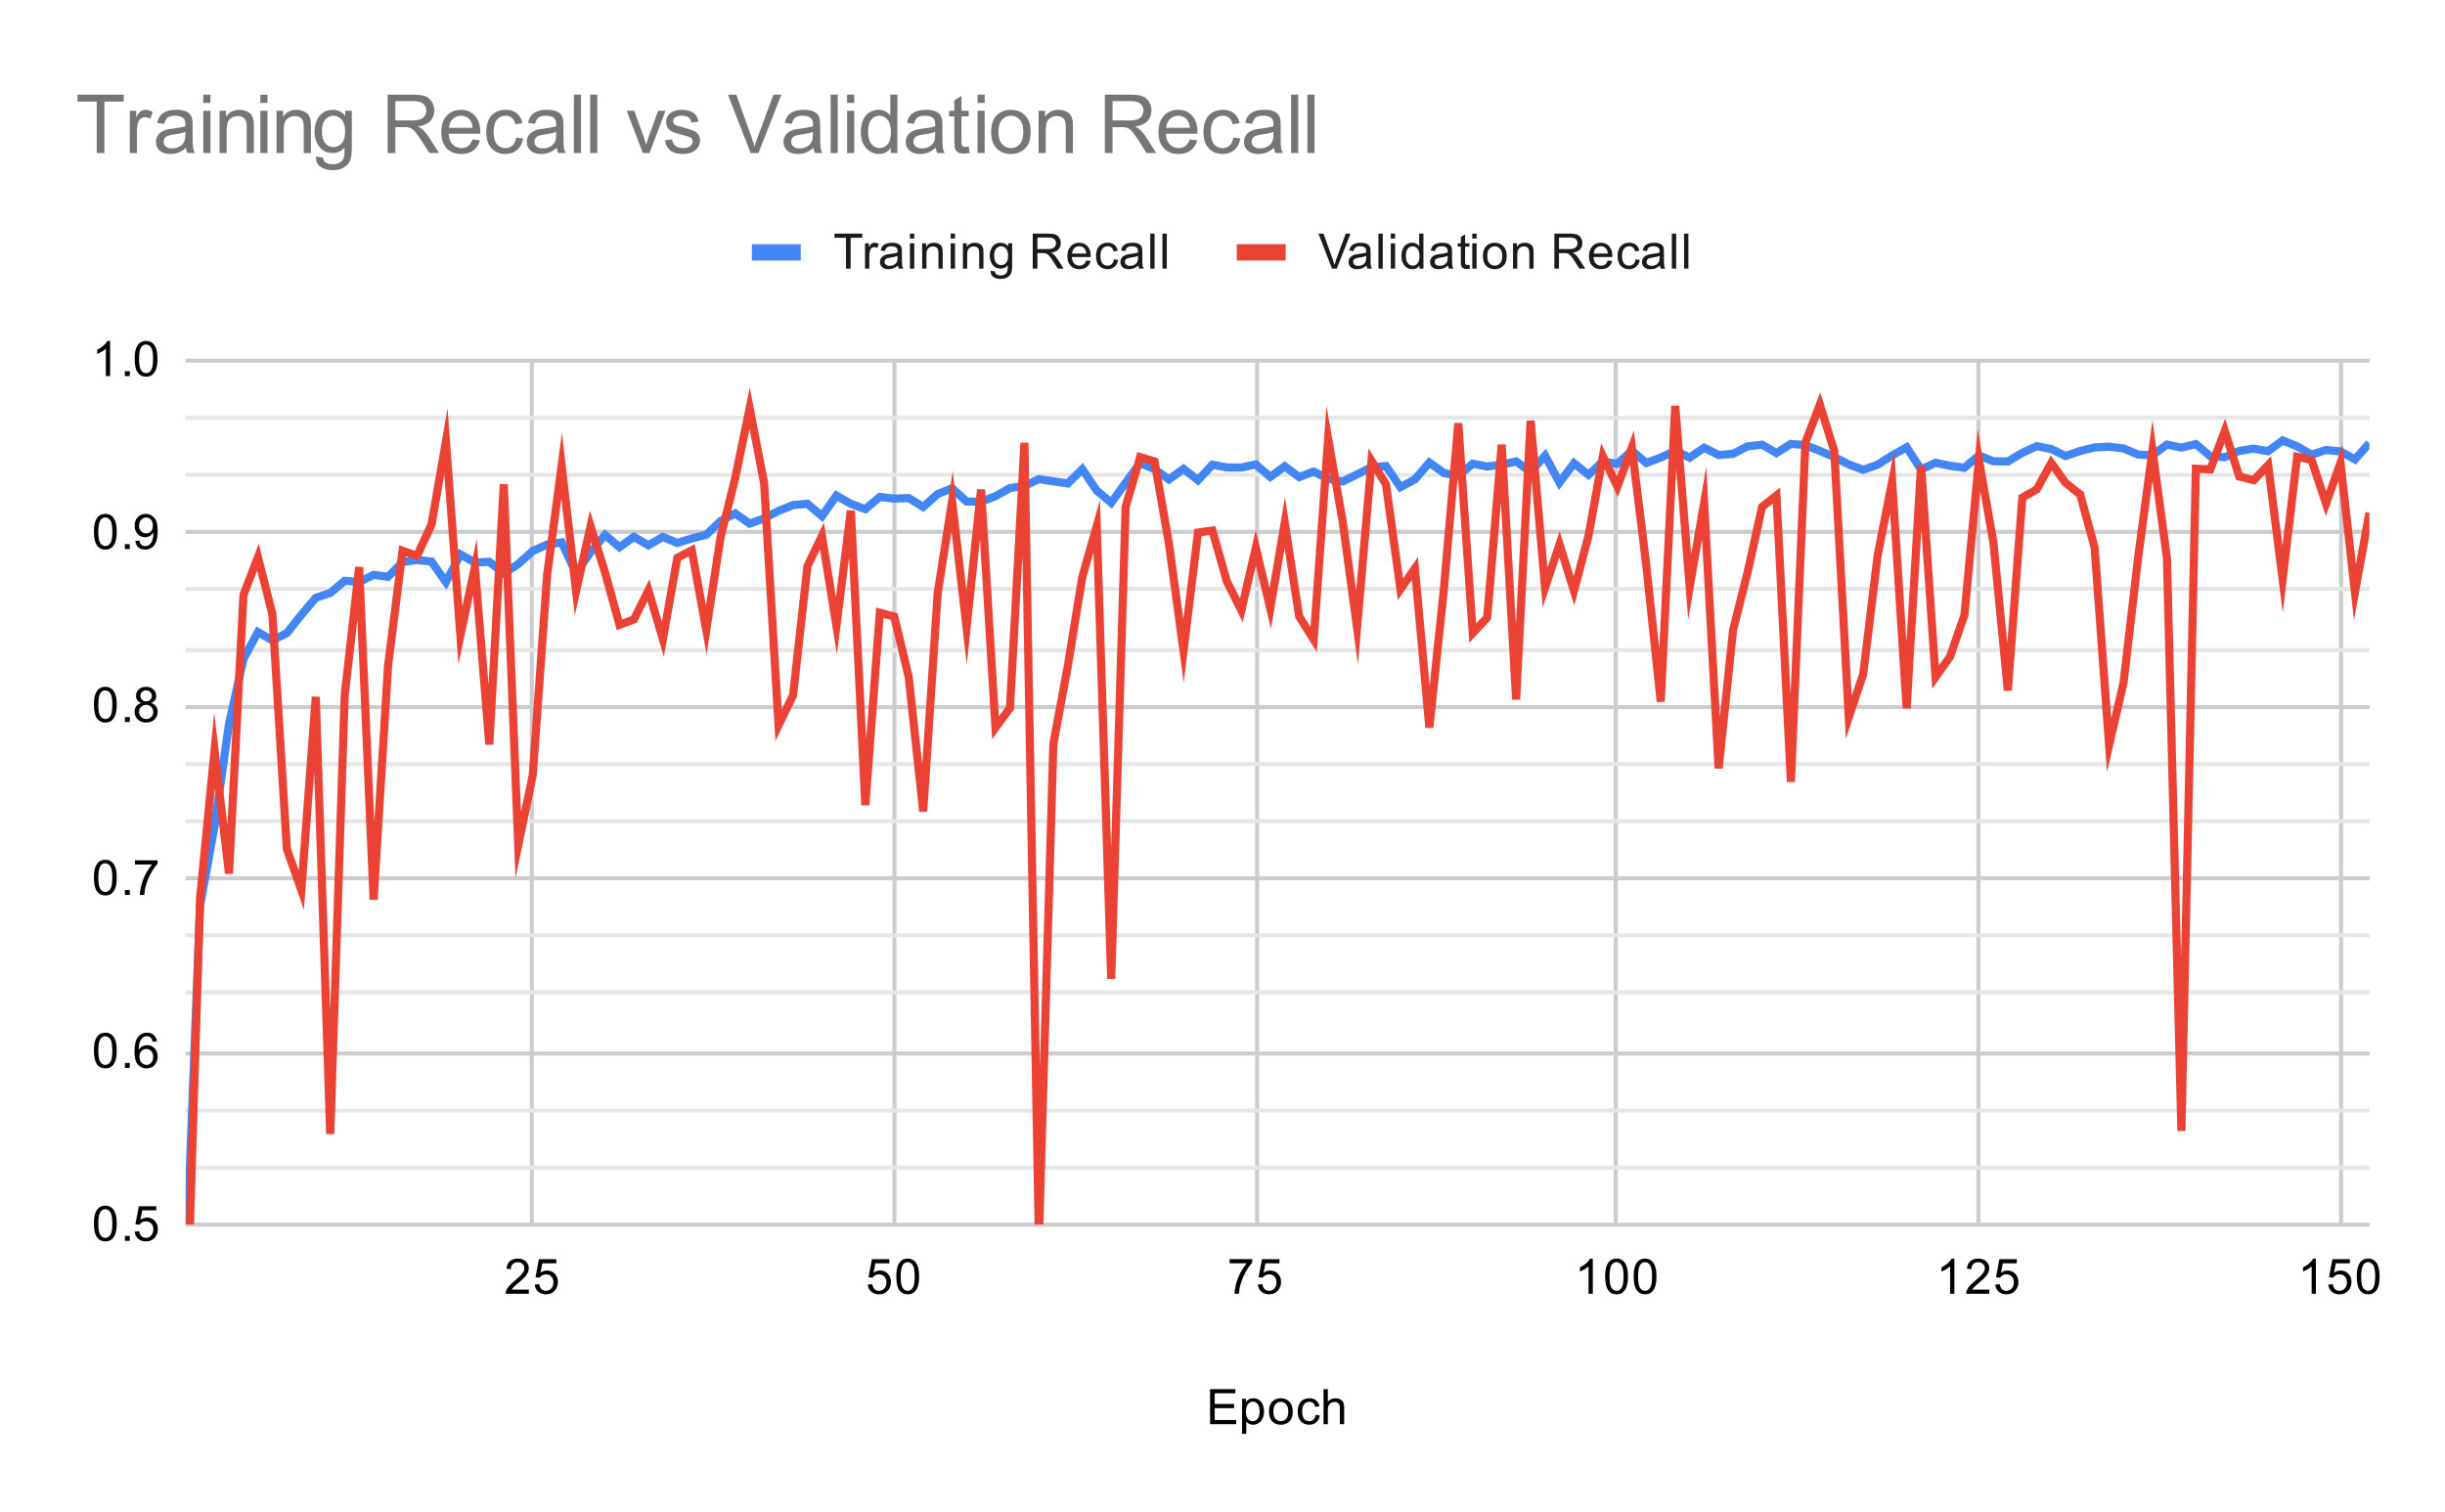
\includegraphics[width=0.3\textwidth]{figs/Project Charts/Training Recall vs Validation Recall.jpg} &
    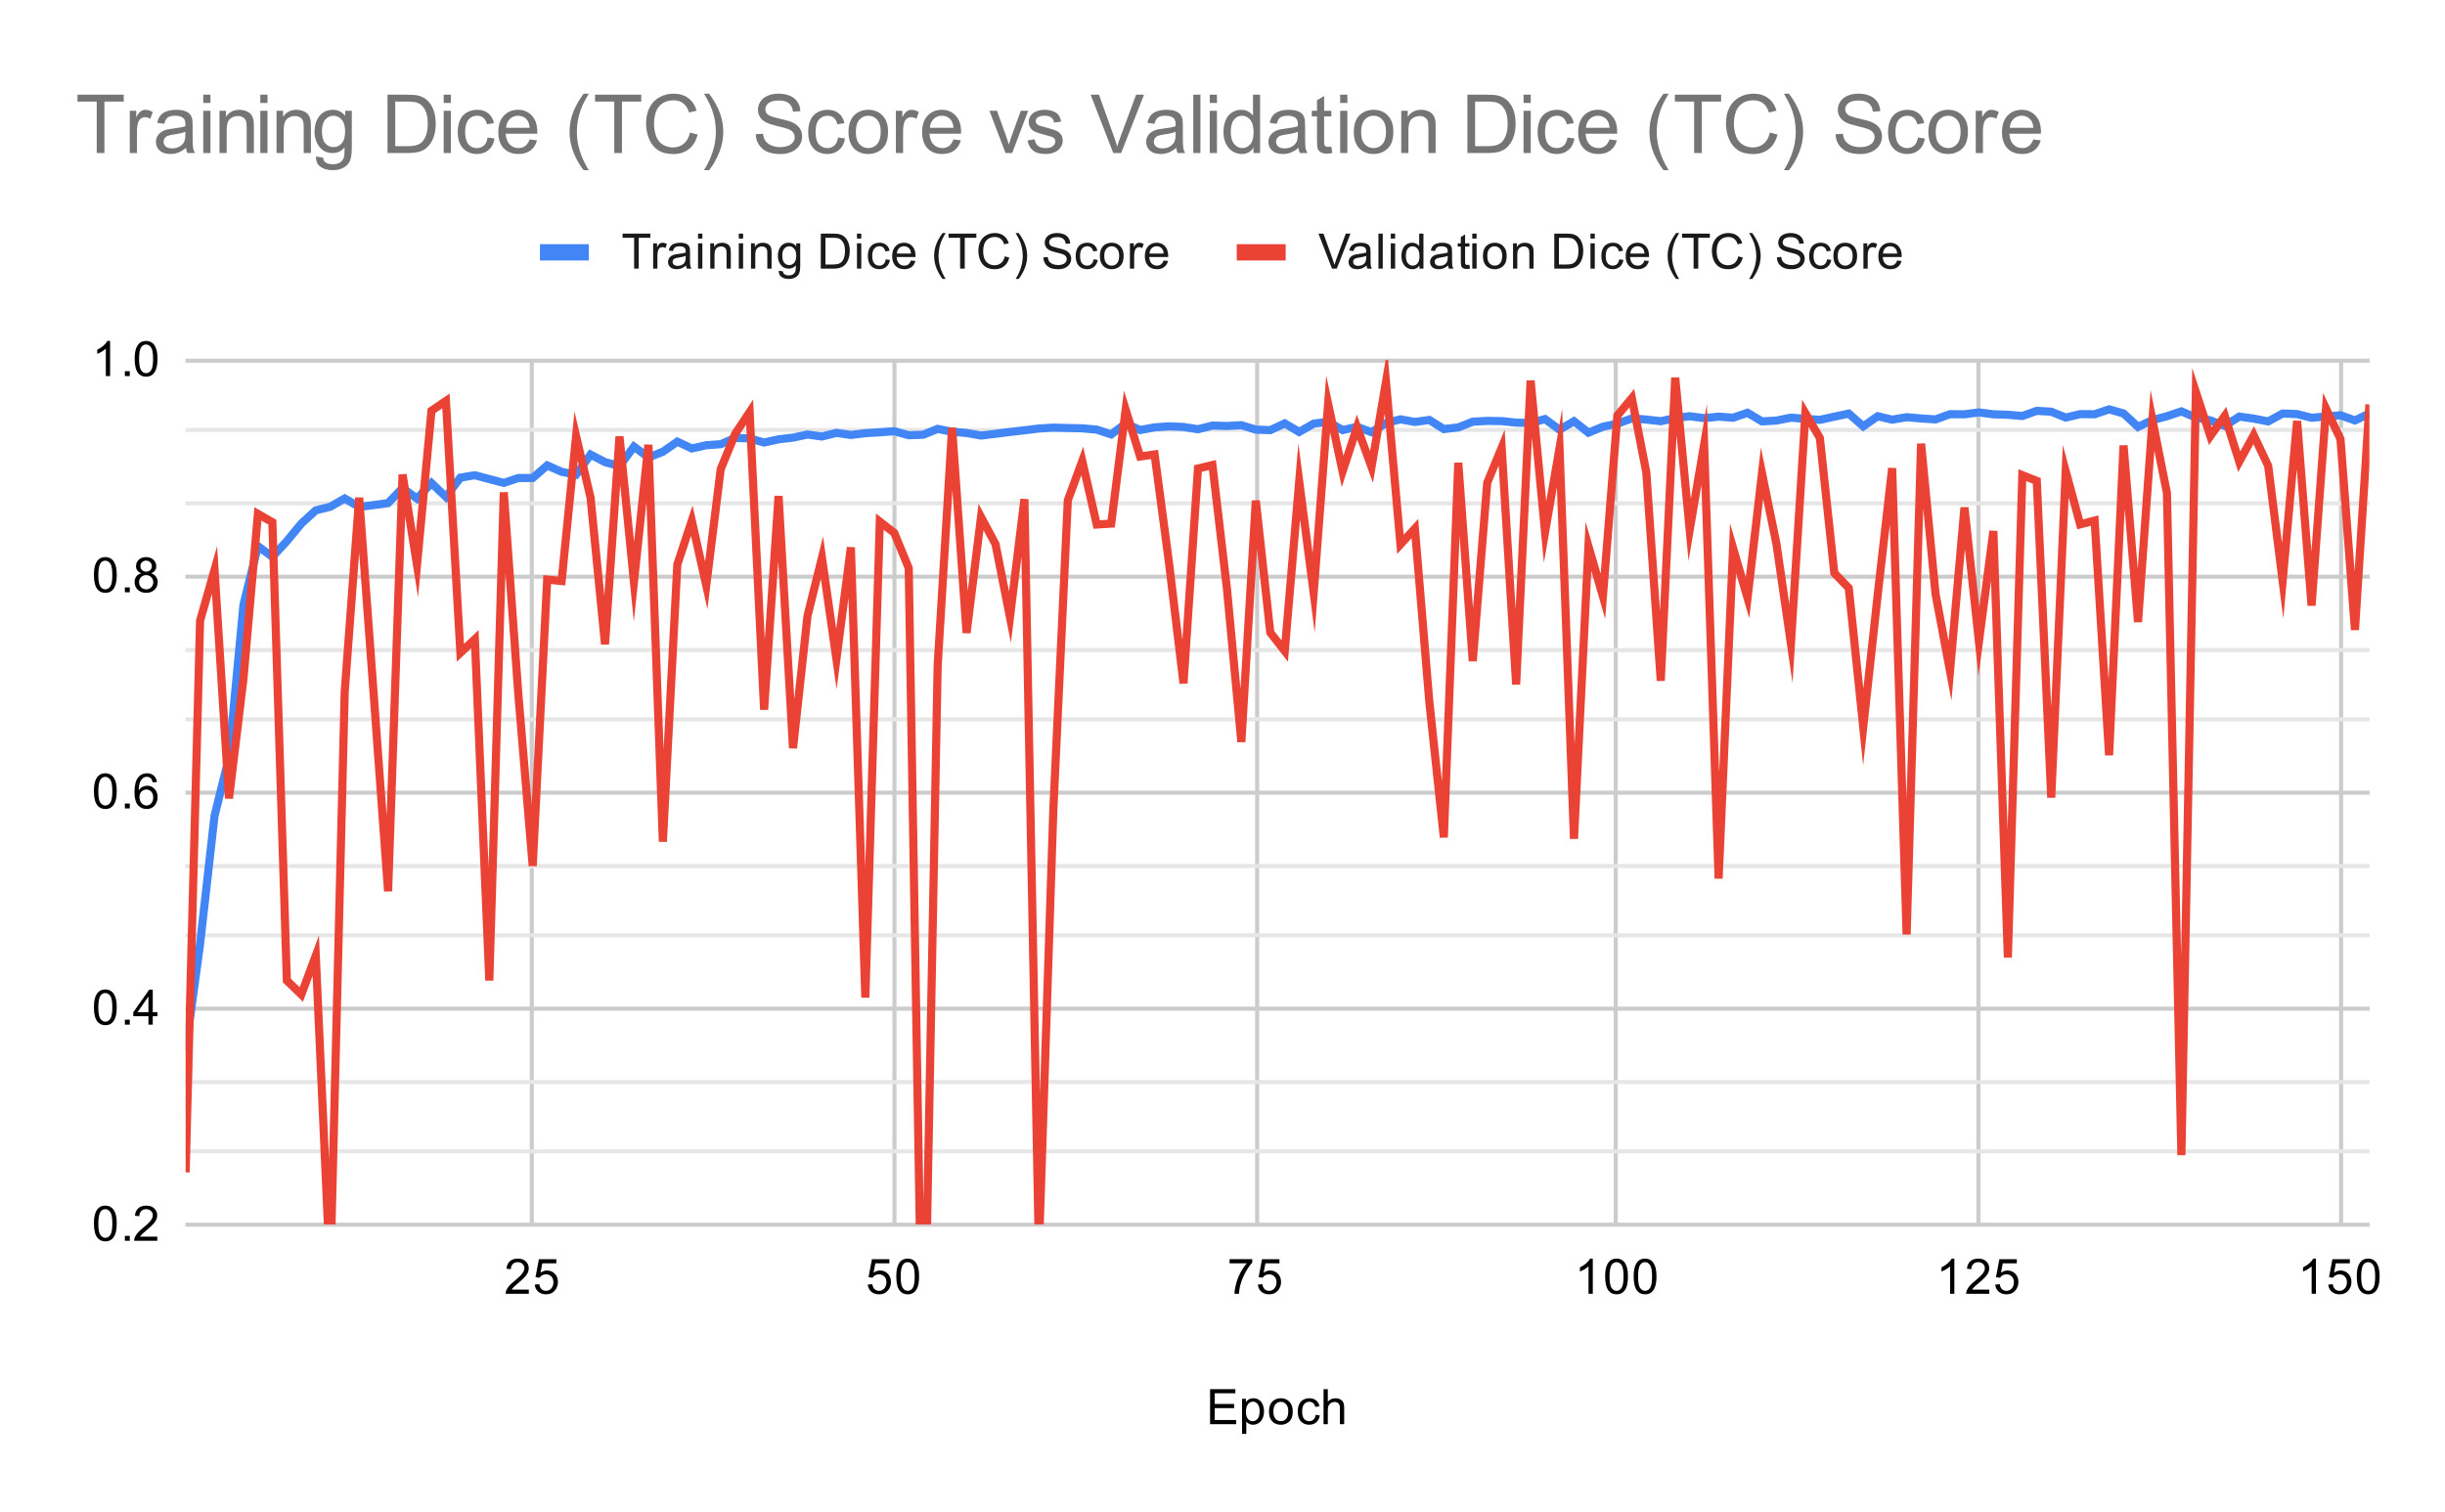
\includegraphics[width=0.3\textwidth]{figs/Project Charts/Training Dice (TC) Score vs Validation Dice (TC) Score.jpg} &
    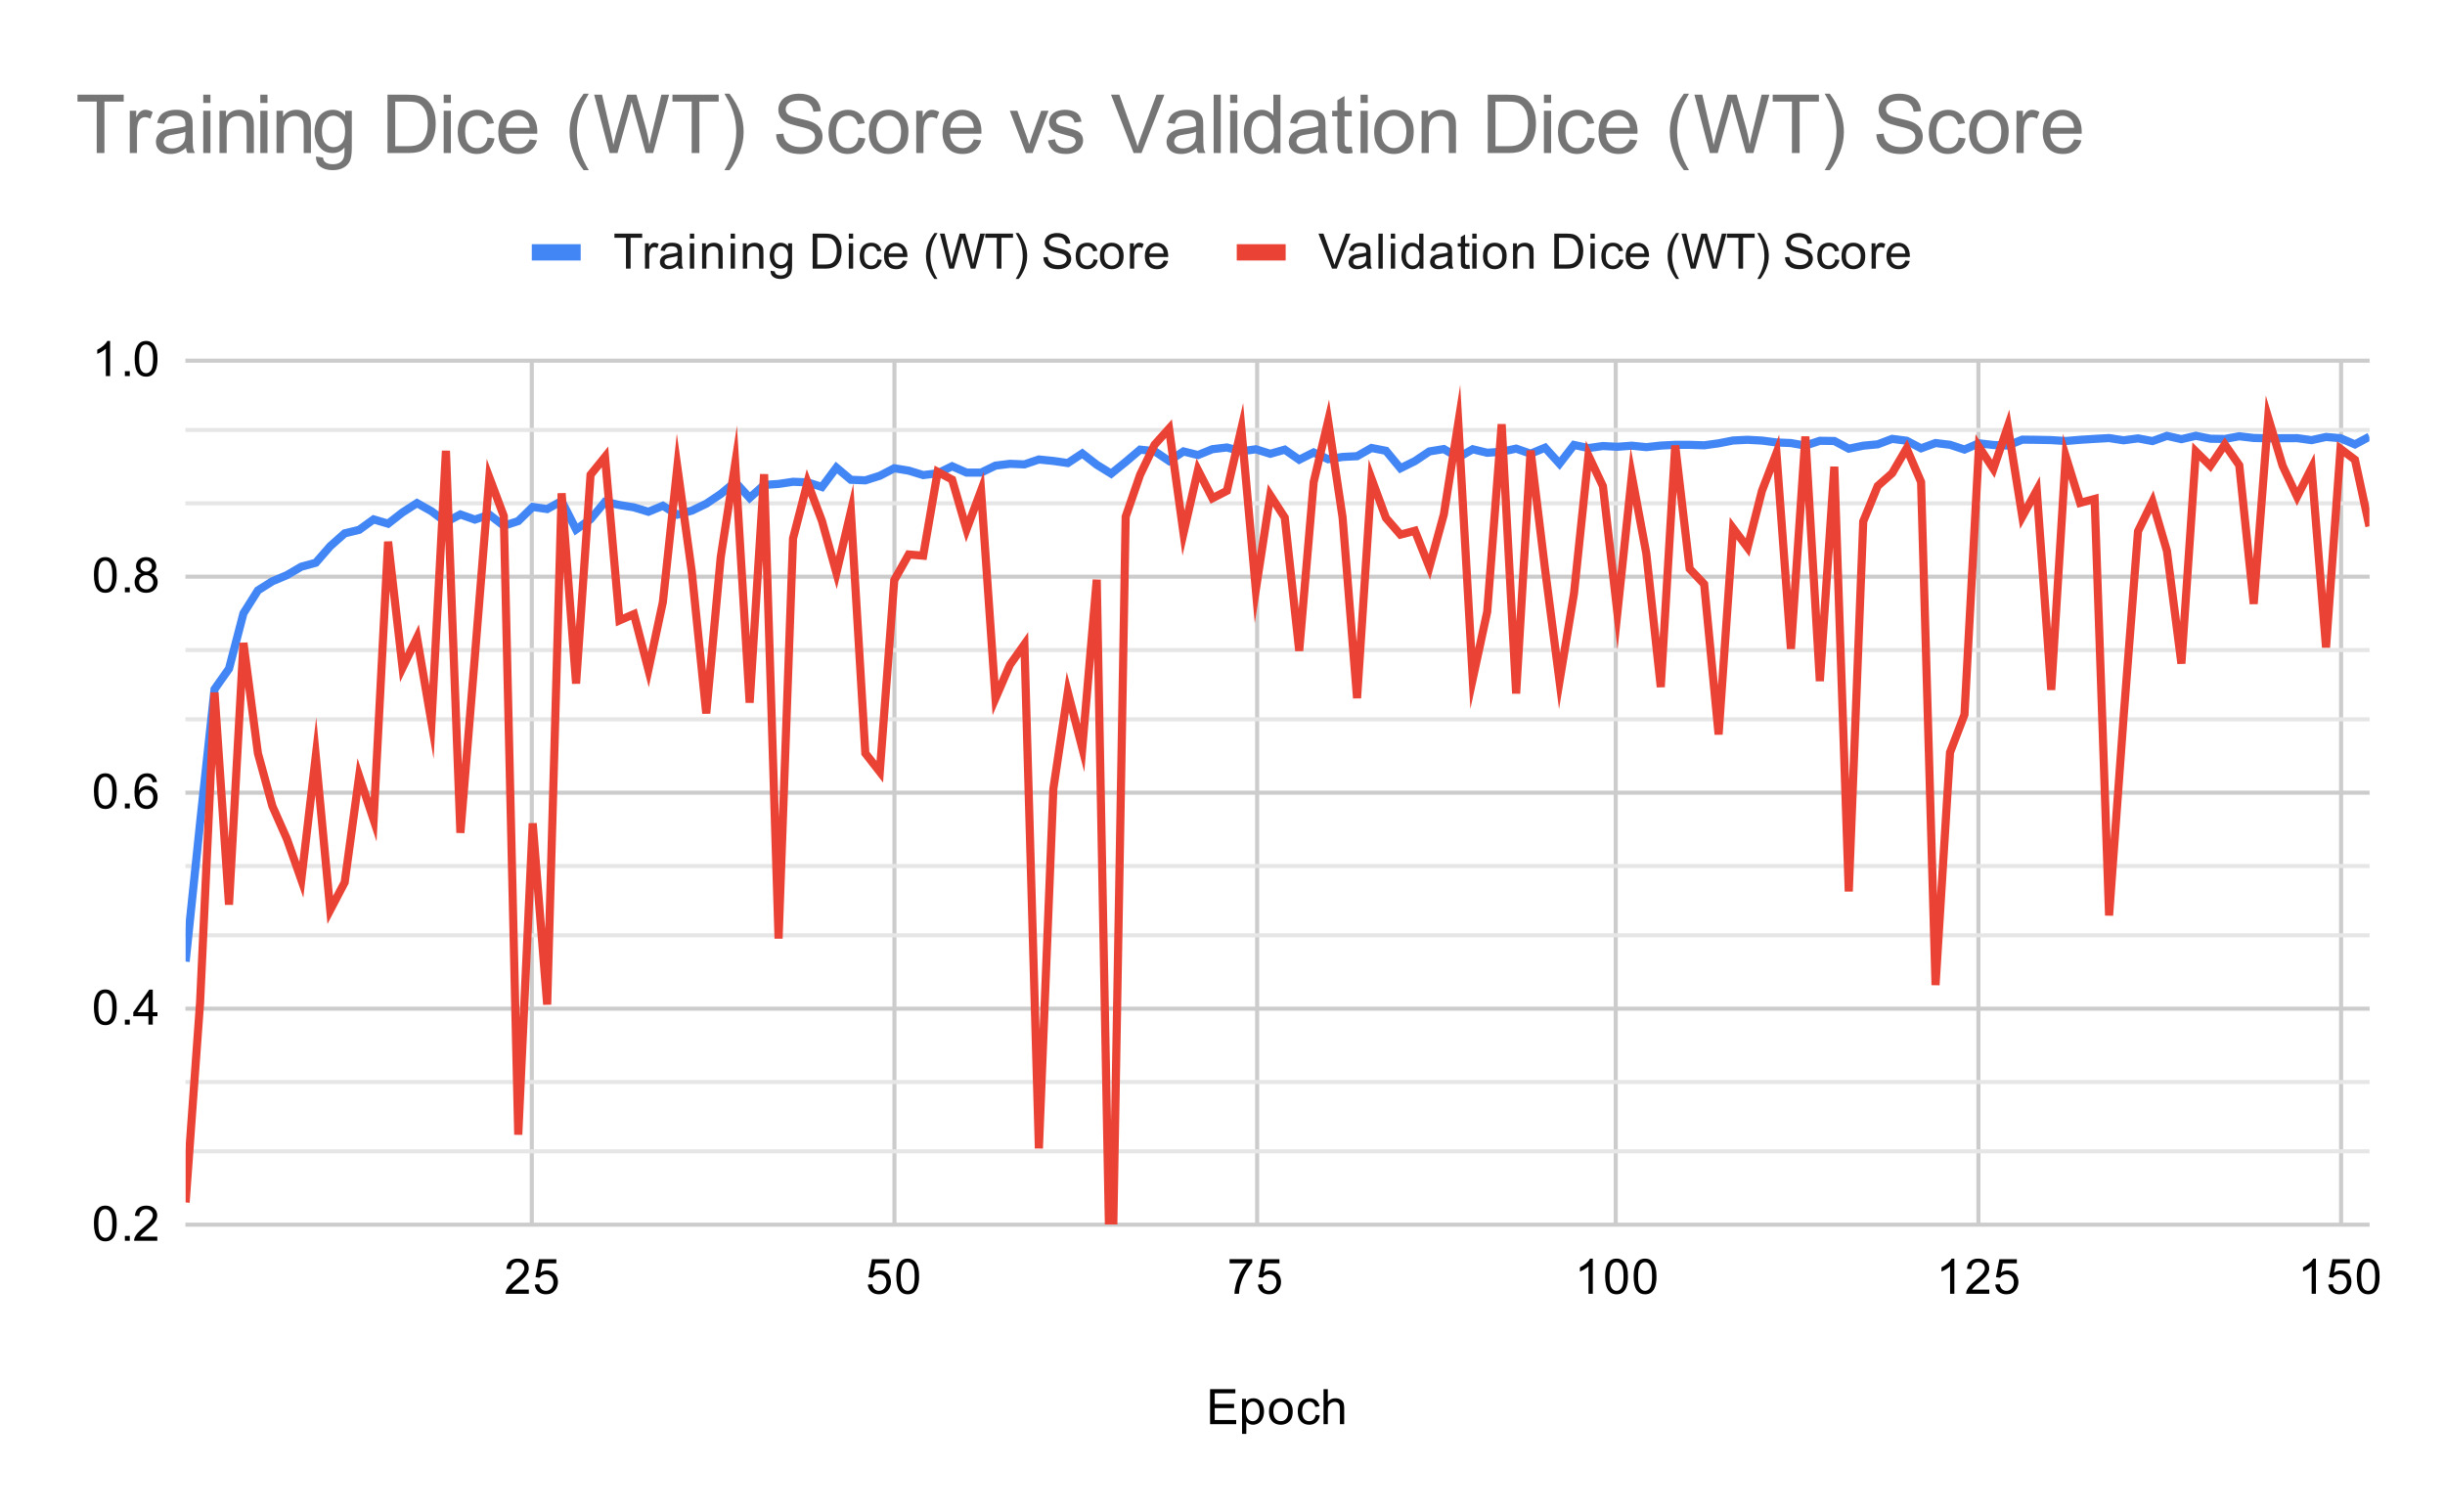
\includegraphics[width=0.3\textwidth]{figs/Project Charts/Training Dice (WT) Score vs Validation Dice (WT) Score.jpg} \\

    (g) Recall Graph & (h) TC Dice Score Graph & (i) WT Dice Score Graph \\[6pt]

    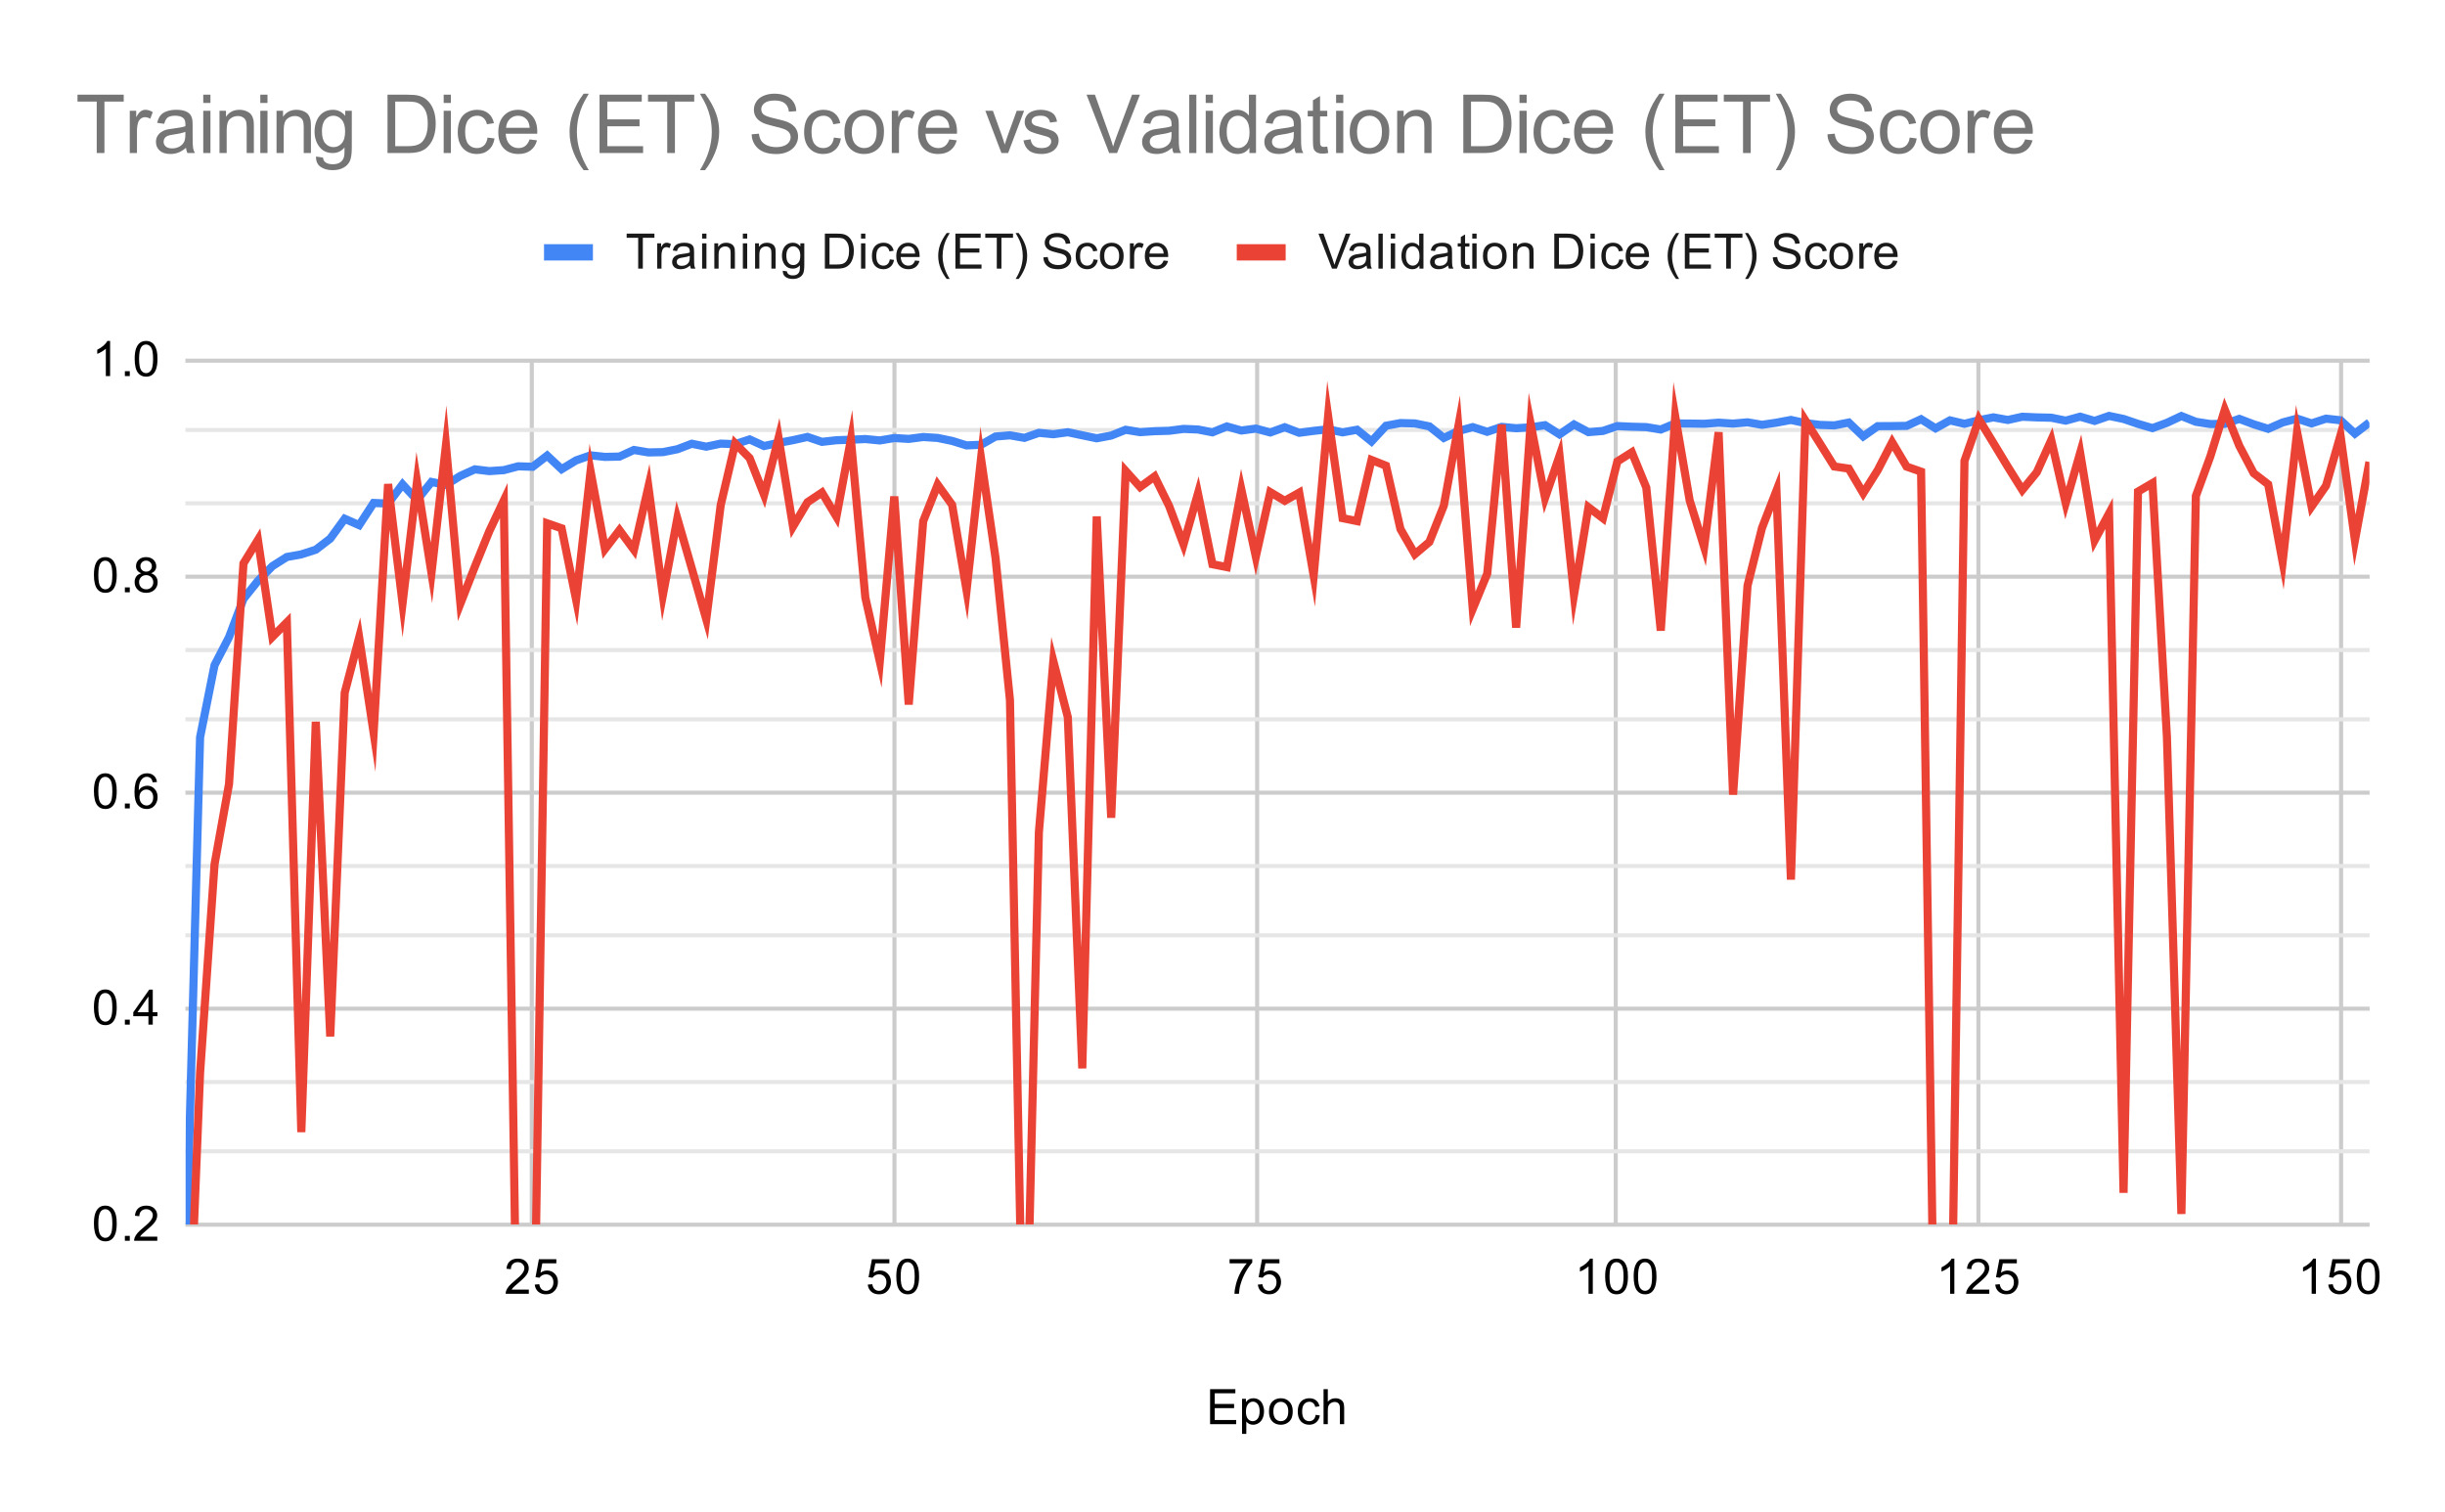
\includegraphics[width=0.3\textwidth]{figs/Project Charts/Training Dice (ET) Score vs Validation Dice (ET) Score.jpg} &
    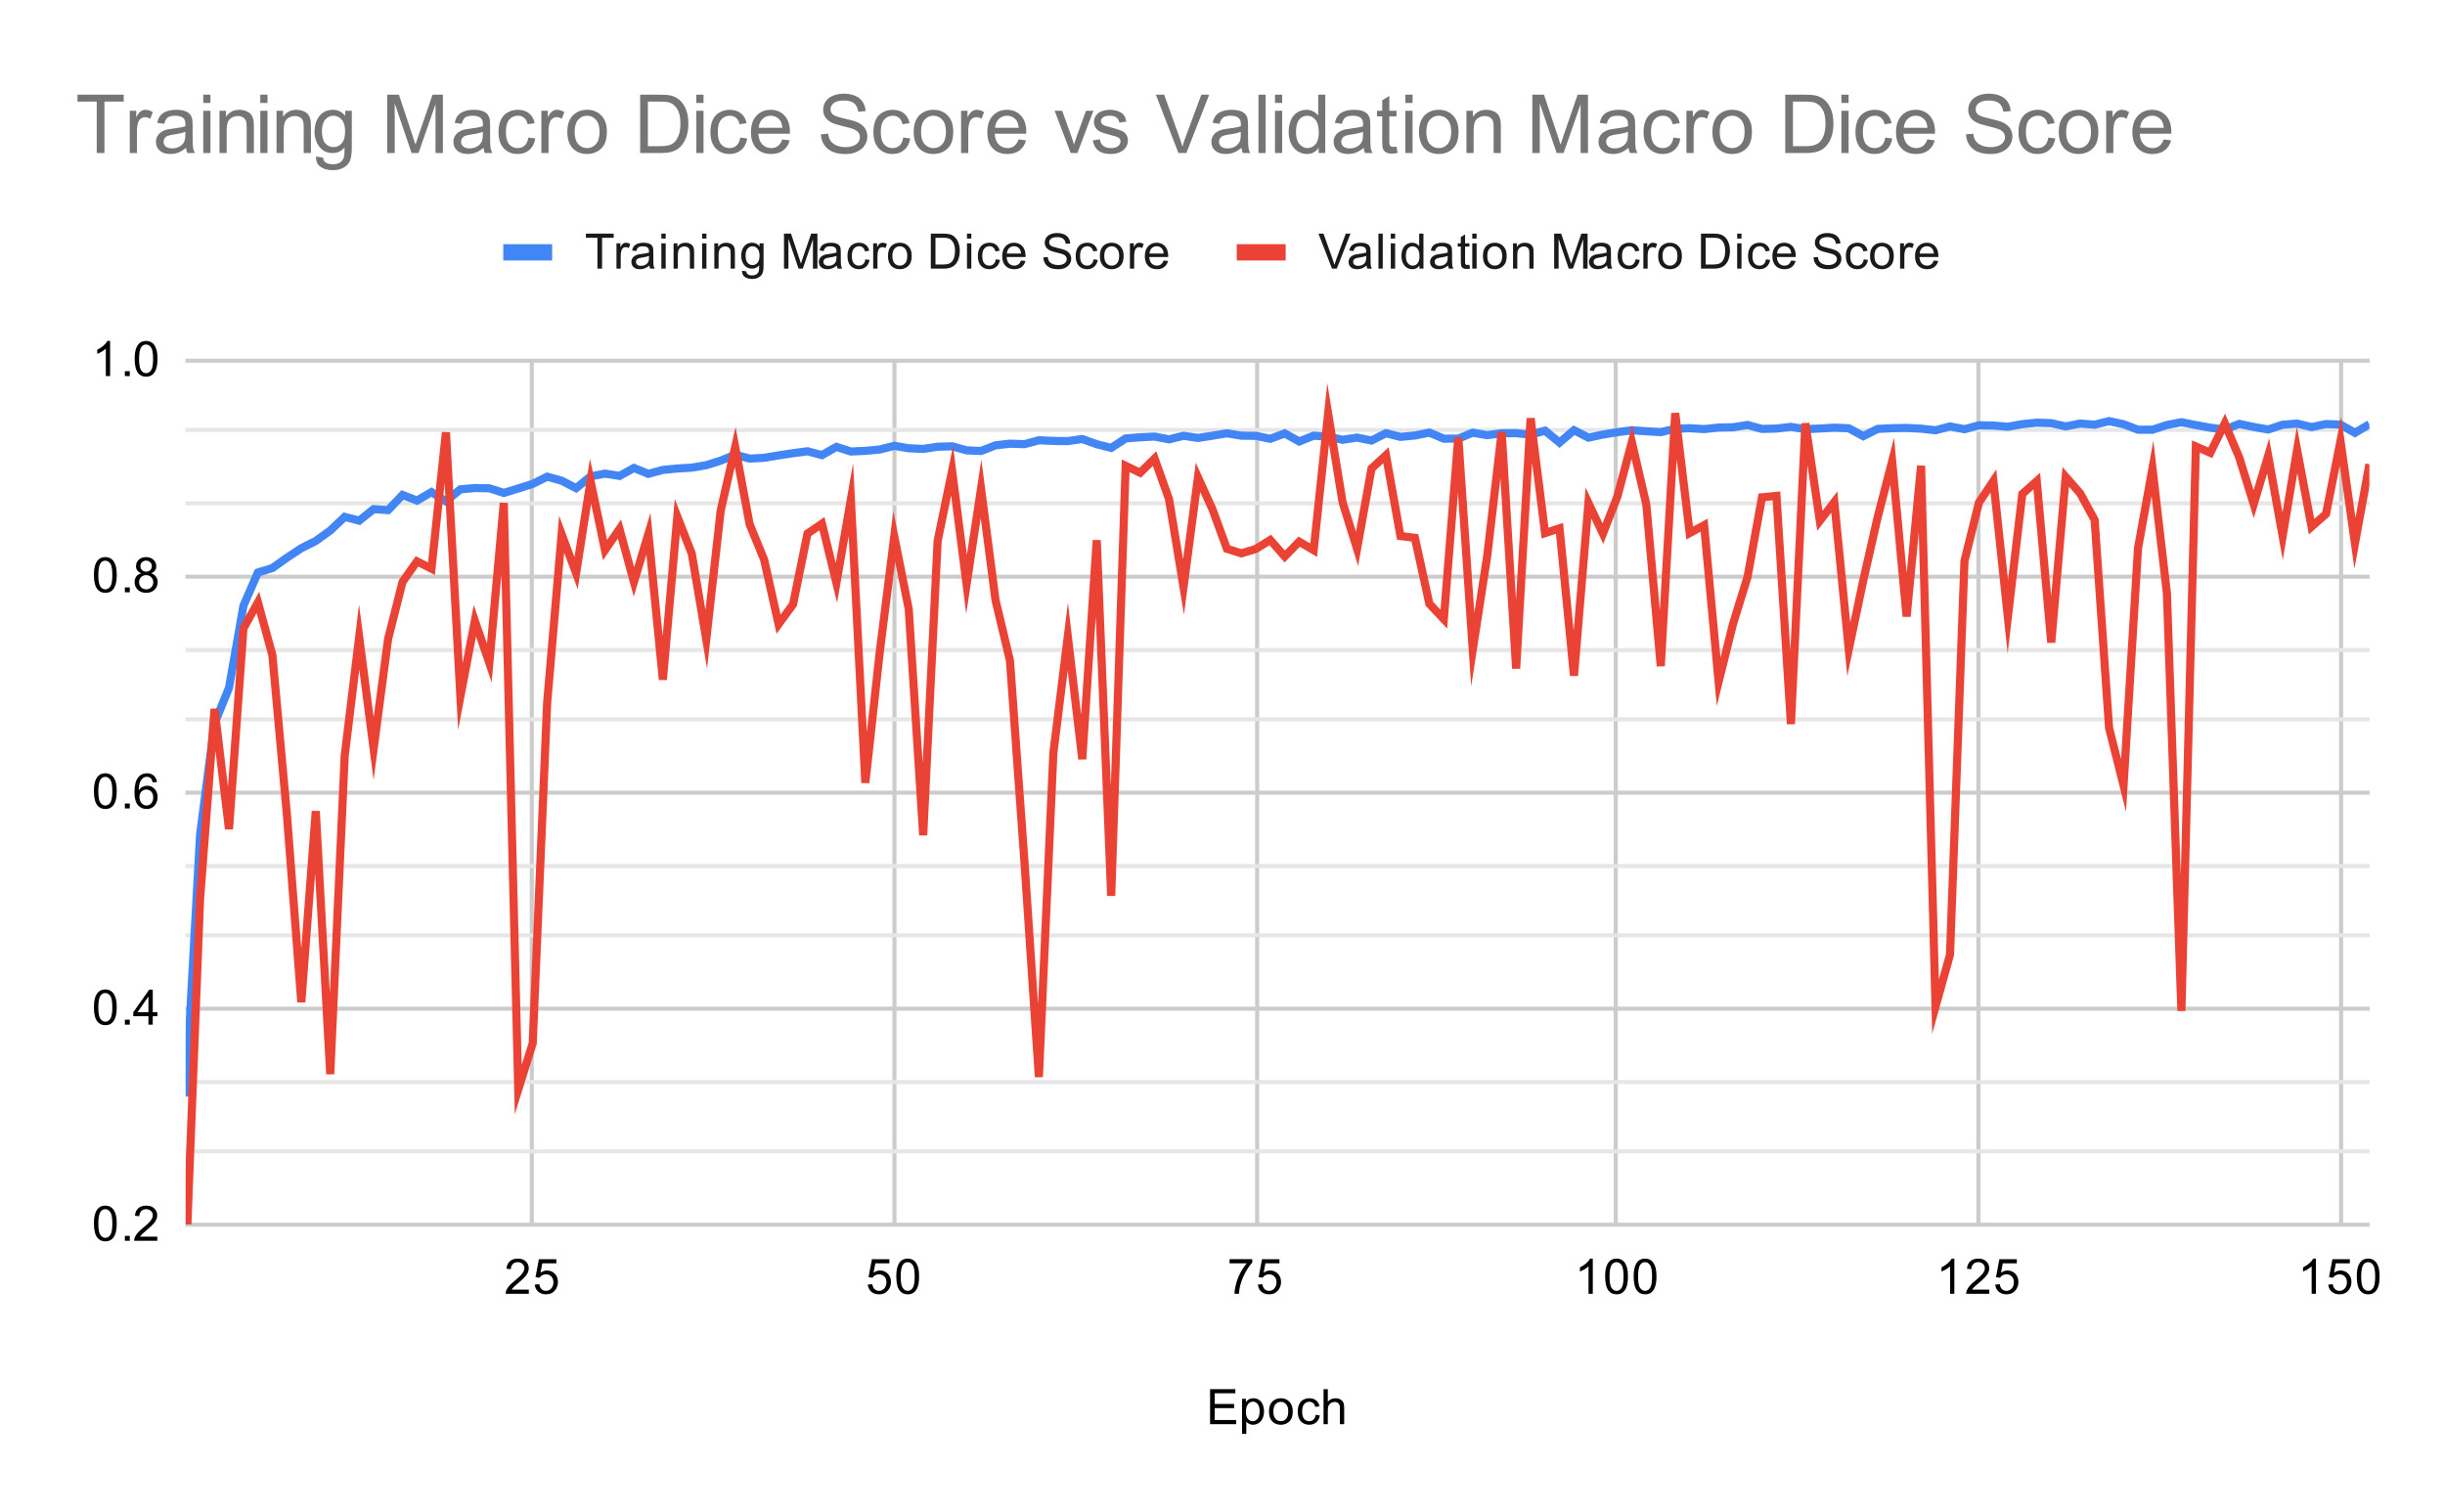
\includegraphics[width=0.3\textwidth]{figs/Project Charts/Training Macro Dice Score vs Validation Macro Dice Score.jpg} & \\

    (j) ET Dice Score Graph & (k) Macro Dice Score Graph &

    \end{tabular}

    \caption{Performance graphs across different evaluation metrics (Training represented as Blue and Validation represented as Red).}
    \label{fig:5x2_graphs}

\end{figure*}

\subsection{Quantitative and Qualitative Analysis}

We evaluated our proposed U-Net variant on the merged BraTS 2020 and 2021 training sets. A 75/25 split was applied, with 25\% of the cases held out for validation. Each case included four co-registered MRI modalities—T1, T1Gd (post-contrast), T2, and FLAIR—along with voxel-wise labels produced by expert neuro radiologists. Label definitions and pre-processing followed the BraTS challenge conventions.

Training continued up to epoch 152, with validation loss and segmentation metrics tracked throughout. We report both the best values observed during training and the final results at epoch 152. Best values reflect the model's peak capability, which could be recovered through checkpoint selection or ensembling.

The results in Table~\ref{tbl1} show balanced and strong performance across tumor subregions, with the highest stability for the Tumor Core (TC) and consistently solid scores for the Enhancing Tumor (ET). Dice WT showed a larger gap between the best and final, highlighting greater sensitivity to checkpoint selection and training dynamics. The best performance the model provides is for the TC region which confirms our proposed dense residual-inception blocks and attention modules are well capable of robust segmentation. The achieved dice score for ET and WT being 0.9055 and 0.8459 respectively and their peak being 0.9538 and 0.9466 shows that model is well capable of segmenting small and heterogeneous classes, but we need to be better at checkpoint selection rather than training the model for a set amount of epochs.

The graphical representations corresponding to each result are provided in Figure~\ref{fig:5x2_graphs} for clarity.

For qualitative assessment, representative segmentation results generated by the final trained model are presented in Figure~\ref{fig:5x2_graphs1}.

\begin{figure*}[!htbp]
    \centering
    \begin{tabular}{ccc}
    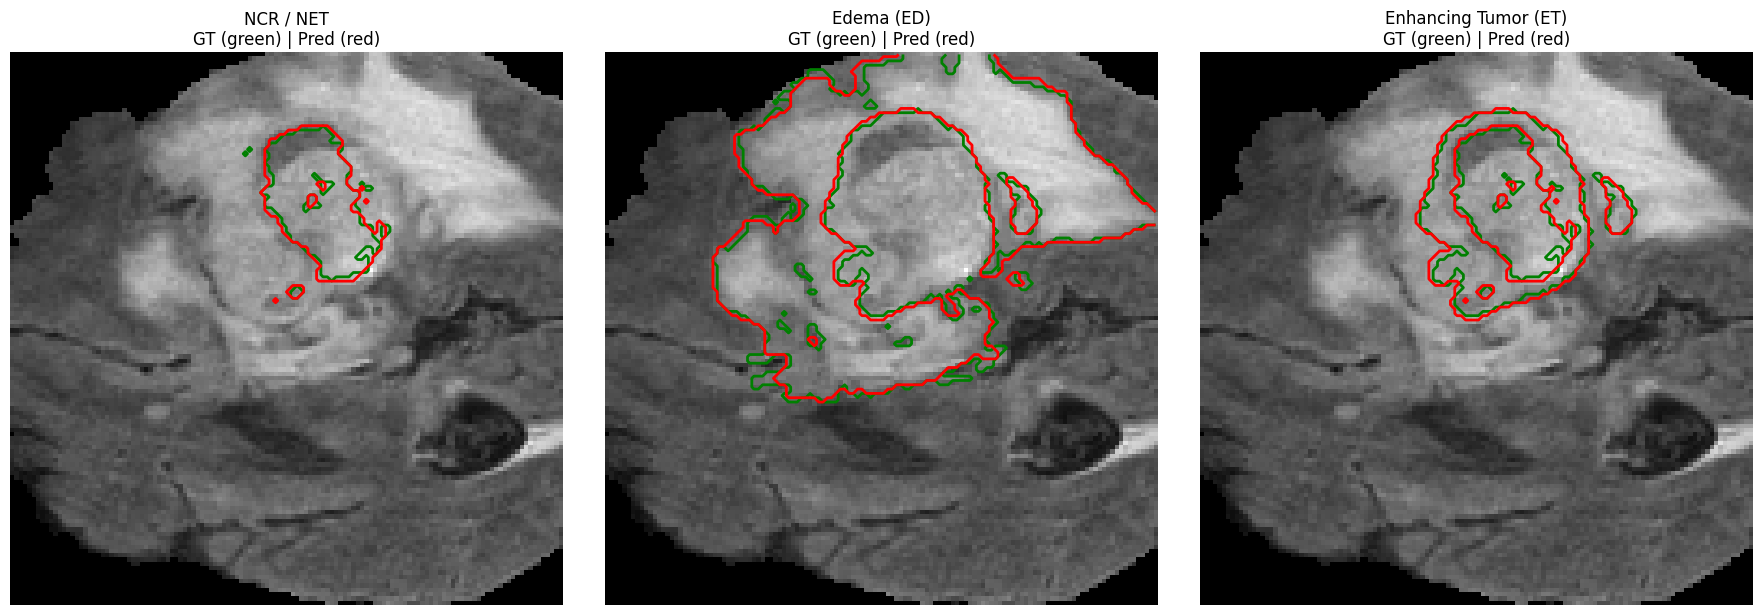
\includegraphics[width=0.30\textwidth]{figs/Conture of Tumor Over Flair images/Image 0.png} &
    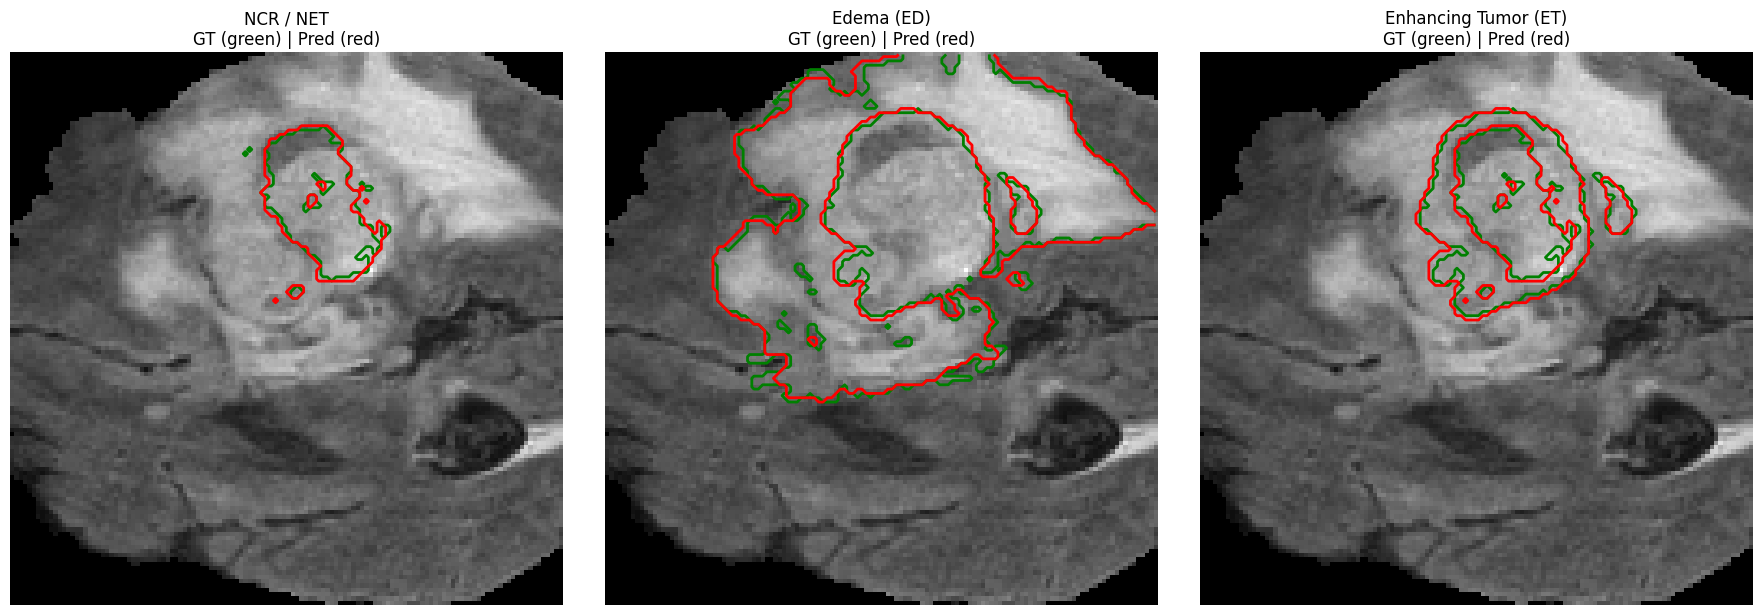
\includegraphics[width=0.30\textwidth]{figs/Conture of Tumor Over Flair images/Image 1.png} &
    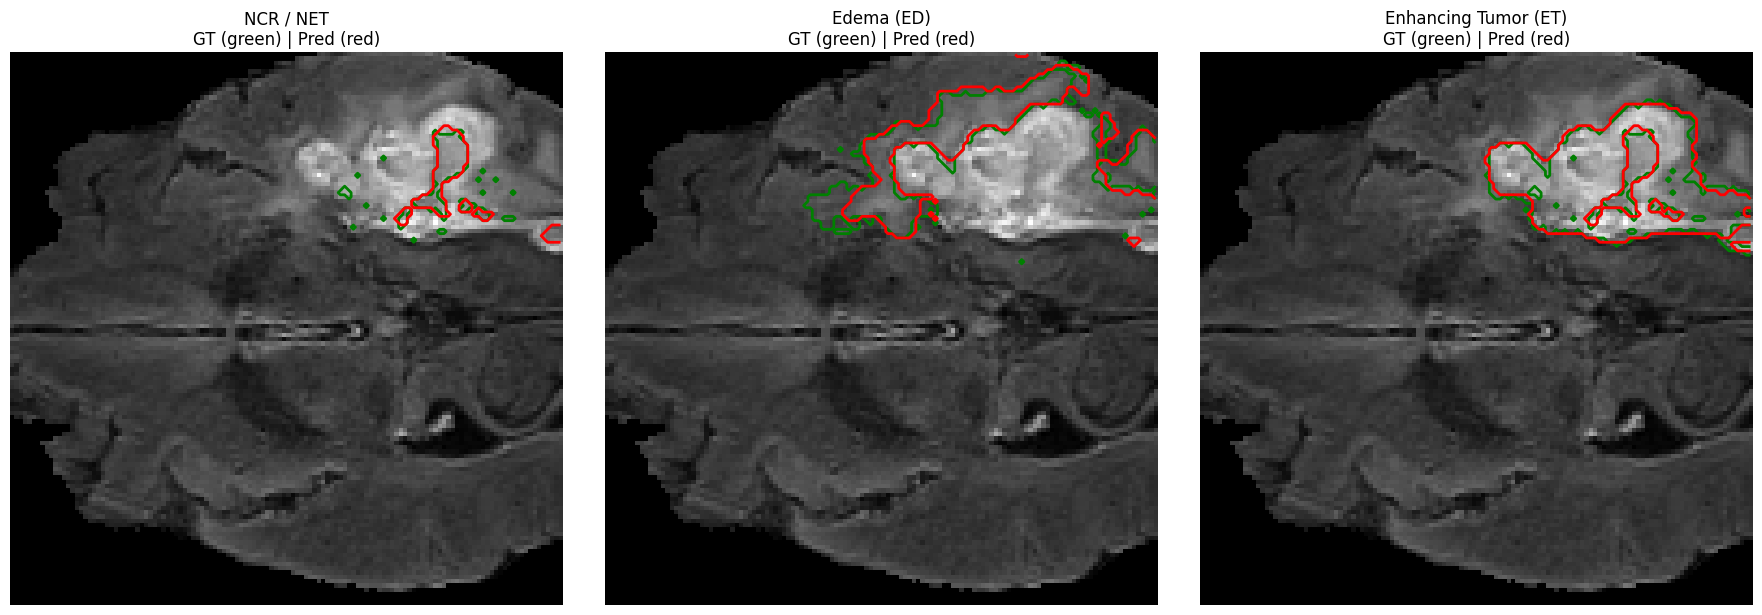
\includegraphics[width=0.30\textwidth]{figs/Conture of Tumor Over Flair images/Image 28.png} \\

    Example 1 & Example 2 & Example 3 \\

    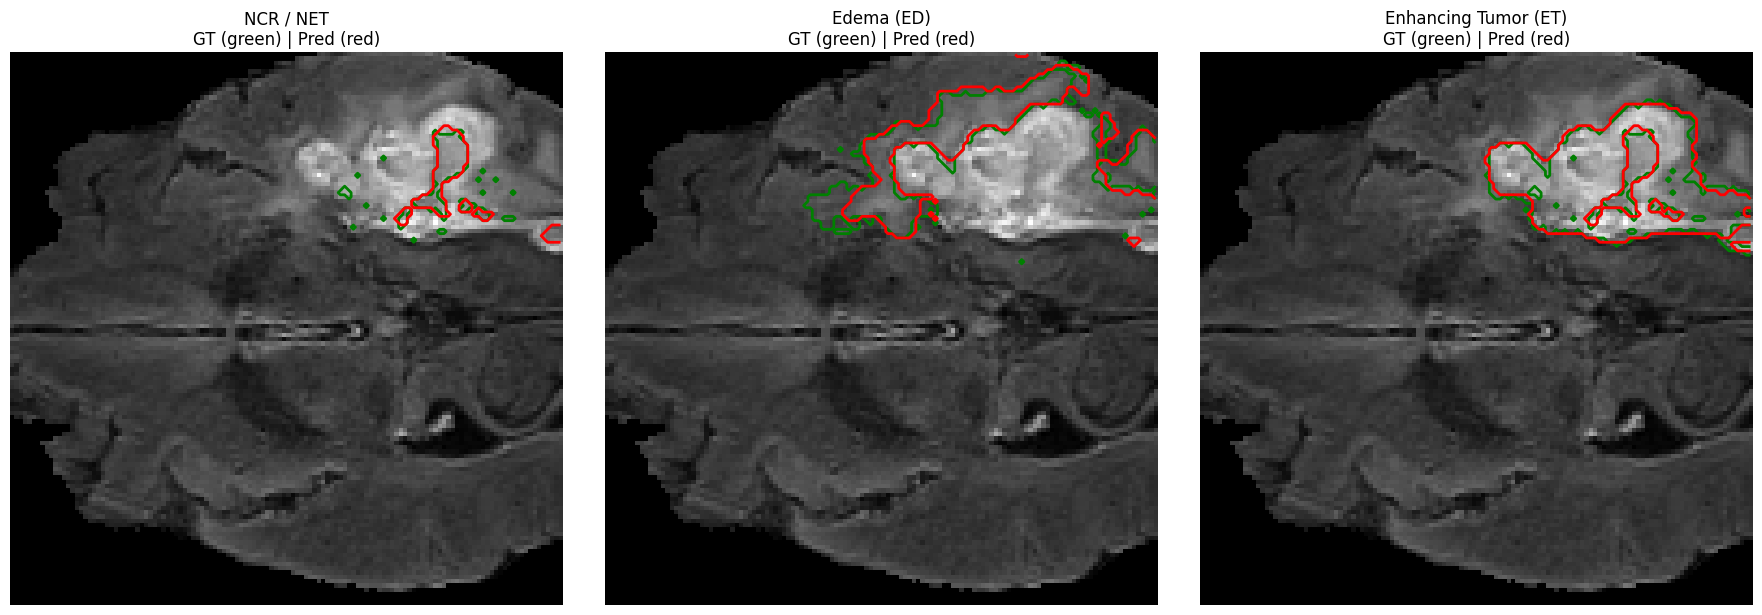
\includegraphics[width=0.30\textwidth]{figs/Conture of Tumor Over Flair images/Image 53.png} &
    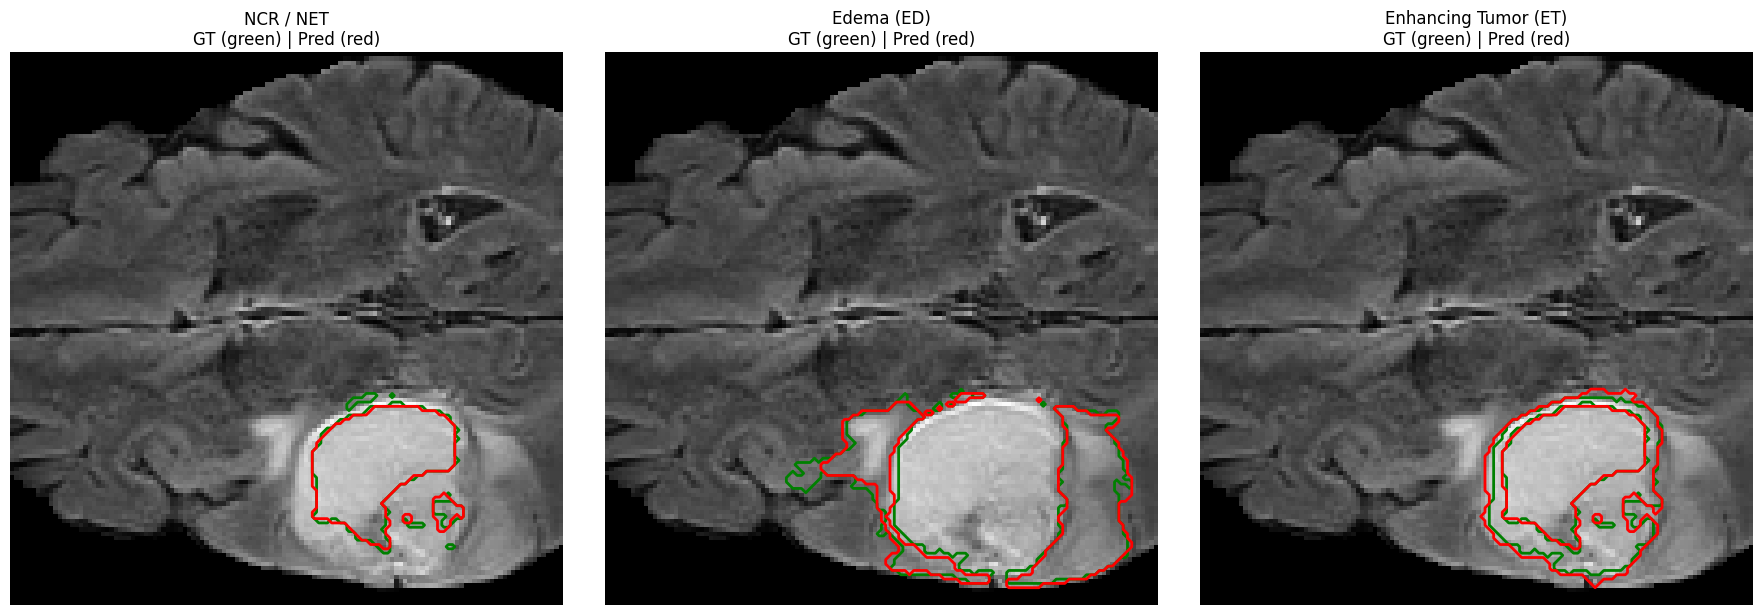
\includegraphics[width=0.30\textwidth]{figs/Conture of Tumor Over Flair images/Image 57.png} &
    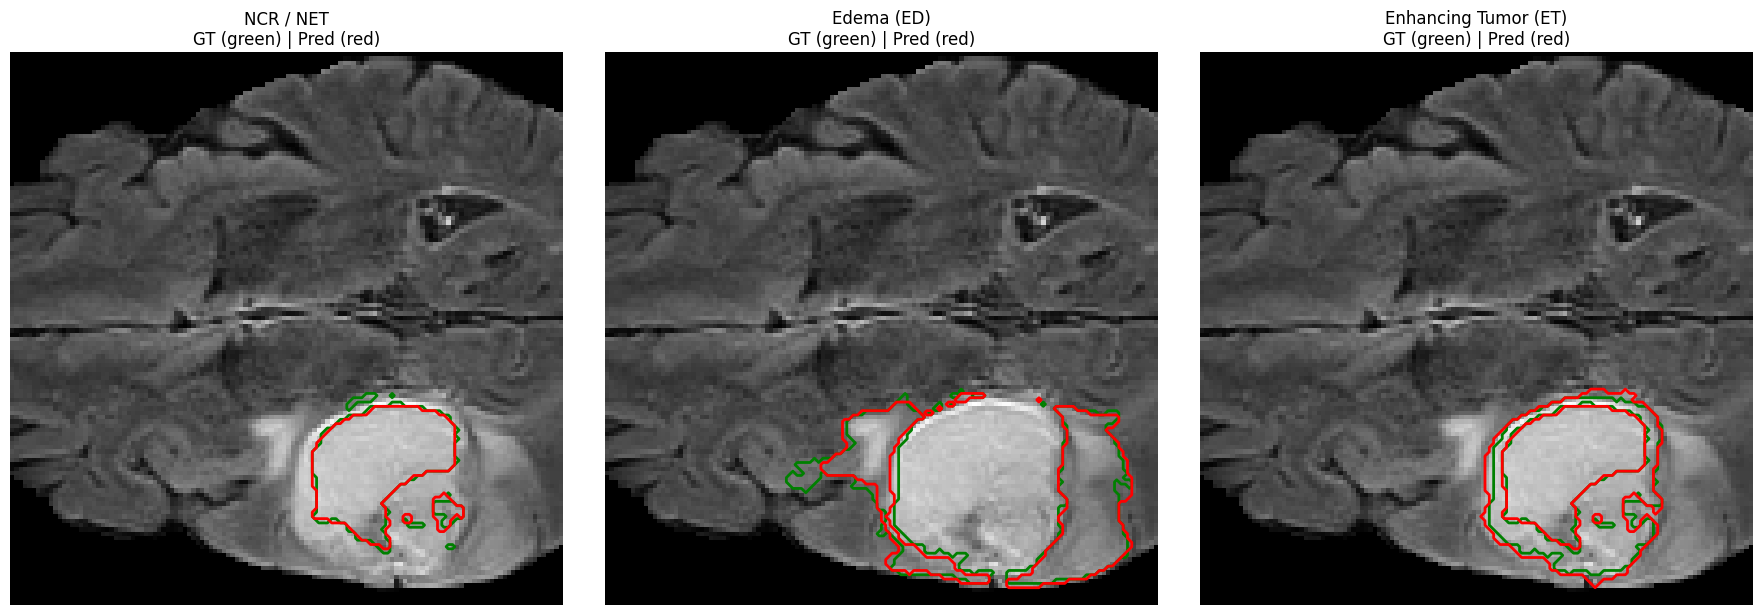
\includegraphics[width=0.30\textwidth]{figs/Conture of Tumor Over Flair images/Image 59.png} \\

    Example 4 & Example 5 & Example 6 \\

    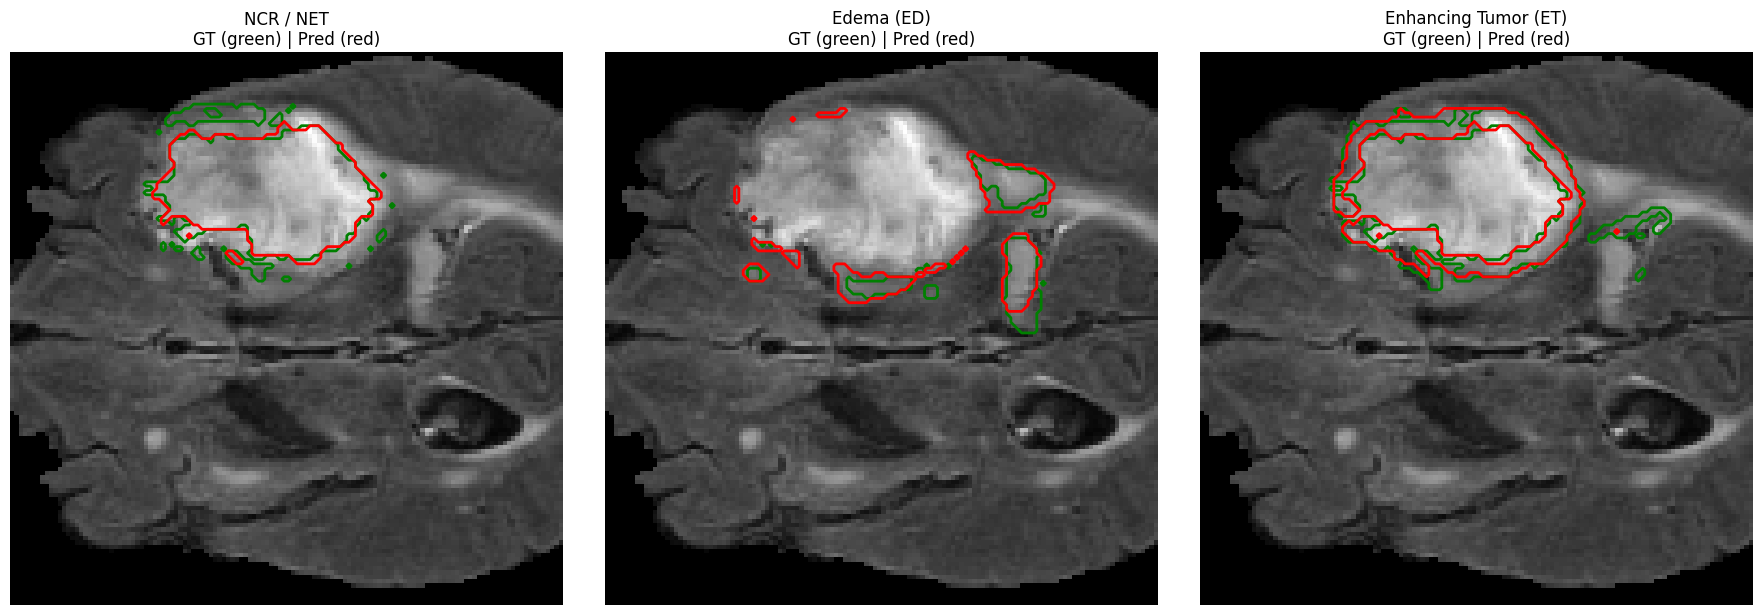
\includegraphics[width=0.30\textwidth]{figs/Conture of Tumor Over Flair images/Image 63.png} &
    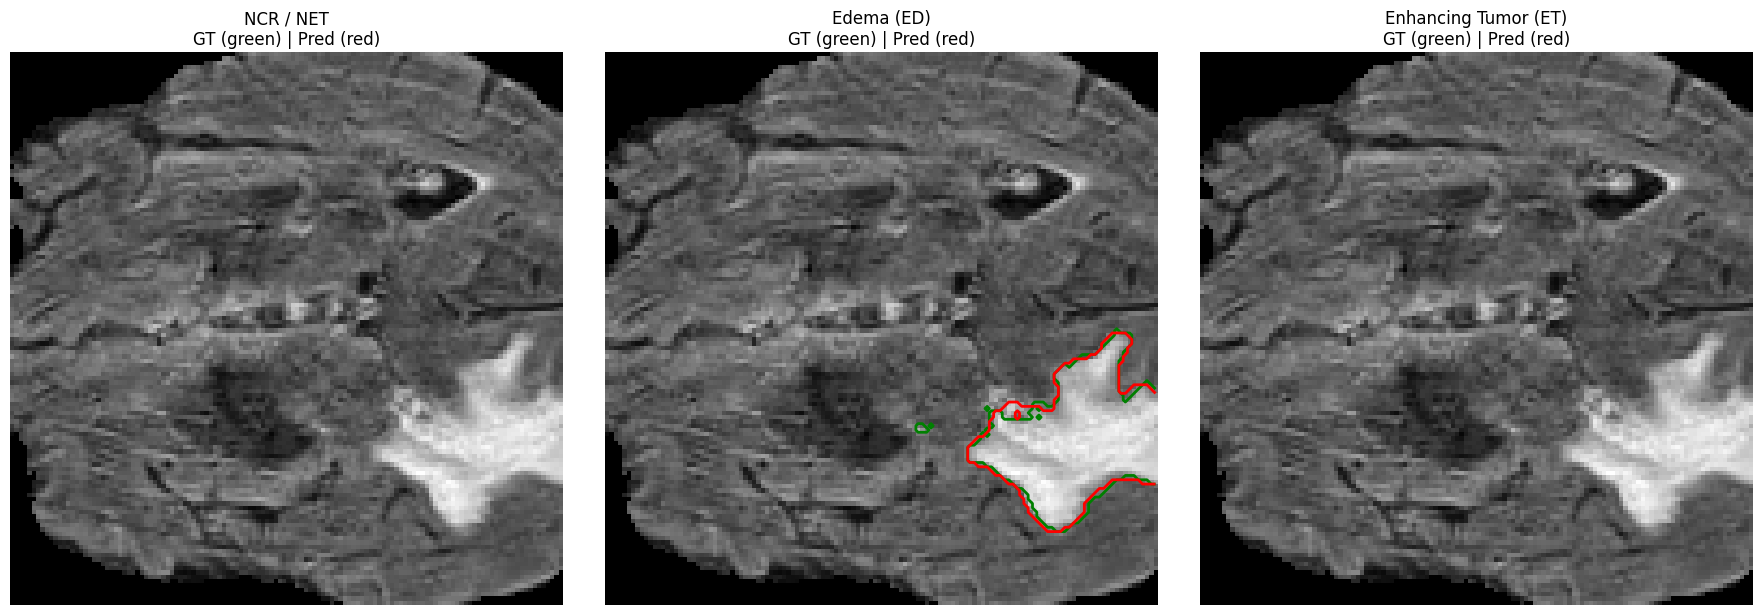
\includegraphics[width=0.30\textwidth]{figs/Conture of Tumor Over Flair images/Image 66.png} &
    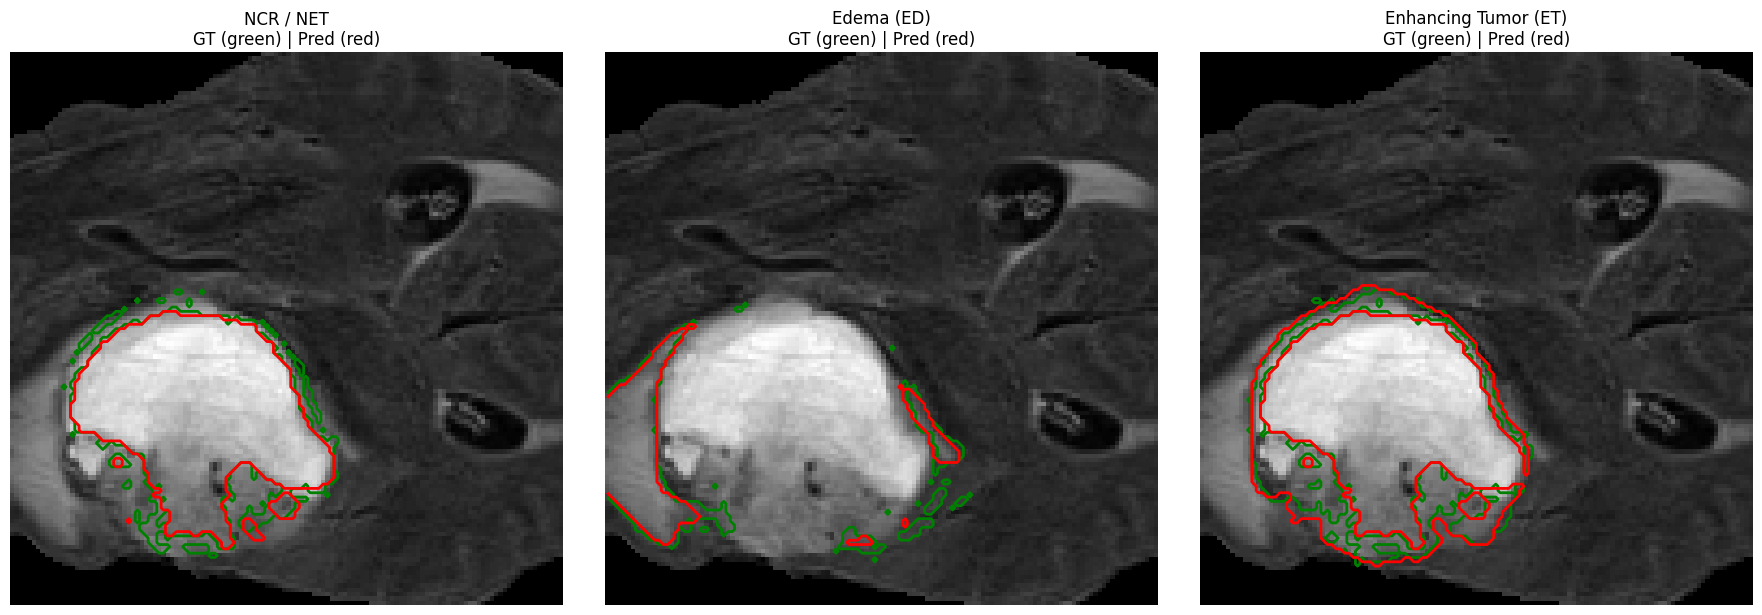
\includegraphics[width=0.30\textwidth]{figs/Conture of Tumor Over Flair images/Image 74.png} \\

    Example 7 & Example 8 & Example 9\\

    \end{tabular}
    \caption{Ground Truth region Conture vs Predicted region Conture for different channels (Ground Truth Represented as Green and Prediction Represented as Red)}
    \label{fig:5x2_graphs1}
\end{figure*}

\subsection{Robustness}

The proposed model is evaluated against other popular network architectures to assess its performance. The comparative results, in Table \ref{tab:brats_comparison}, demonstrate the effectiveness and robustness of the proposed method.

\begin{table*}[!htbp]
    \caption{Comparison of Dice scores on BraTS benchmark datasets.}
    \label{tab:brats_comparison}
    \centering
    \begin{tabular}{lcccc}
        \toprule
        Model (Dataset / Year) & WT Dice & TC Dice & ET Dice & Source \\
        \midrule
        Myronenko (BraTS 2018) & 0.884 & 0.815 & 0.766 & BraTS 2018 Test \\
        Two-Stage Cascaded U-Net (BraTS 2019) & 0.888 & 0.837 & 0.833 & BraTS 2019 Test \\
        nnU-Net (BraTS 2020) & 0.890 & 0.851 & 0.820 & BraTS 2020 Test \\
        TransBTS (2021) & 0.900 & 0.819 & 0.789 & Reported (TTA) \\
        Swin UNETR (2022) & 0.926 & 0.885 & 0.858 & Validation \\
        SwinBTS (2022) & 0.918 & 0.848 & 0.832 & Reported \\
        BiTr-UNet (BraTS 2021) & 0.926 & 0.935 & 0.887 & BraTS 2021 Test \\
        Triplanar Ensemble (BraTS 2020) & 0.890 & 0.840 & 0.810 & BraTS 2020 Test \\
        S3D-UNet (2018) & 0.839 & 0.783 & 0.689 & Reported \\
        Cascaded V-Nets (BraTS 2018) & 0.876 & 0.795 & 0.736 & BraTS 2018 Test \\
        \textbf{Our Model (BraTS 2020+2021)} & \textbf{0.846} & \textbf{0.959} & \textbf{0.906} & 75/25 Validation \\
        \bottomrule
    \end{tabular}
\end{table*}

On validation, our model ranks among top performers for TC and ET, with Dice scores of $0.959$ and $0.906$ respectively. While WT Dice was $0.846$ at the final epoch—slightly lower than models reporting >0.90—our peak WT Dice reached $0.947$, indicating checkpointing or ensembling could close this gap. Overall, the model delivers competitive performance, particularly for TC and ET segmentation, aligning with recent transformer-hybrid models.

\subsection{Computational Complexity}

One notable advantage of the proposed model is its computational efficiency is that it being light-weight. When we compare the parameter count of our model with others we observe the following in Table \ref{tab:parameter_comparison}.

\begin{table*}[!htbp]
    \caption{Comparison of total trainable parameters across recent 3D segmentation models.}
    \label{tab:parameter_comparison}
    \centering
    \begin{tabular}{lcc}
        \toprule
        Model (Ref.) & Total Parameters (M) & Remarks \\
        \midrule
        \textbf{Our Model (this work)} & \textbf{4.01} & All parameters trainable \\
        SegFormer3D (2024) & 4.50 & Lightweight transformer \\
        LightM-UNet & 5.02 & Lightweight baseline \\
        3D U-Net & 16.21 & Canonical 3D configuration \\
        VT-UNet-B & 20.80 & Transformer-based encoder \\
        TransBTS (2021) & 32.99 & CNN + Transformer hybrid \\
        nnU-Net (default) & $\sim$30.00 & Dataset-dependent configuration \\
        nnFormer & 39.70 & Hierarchical transformer \\
        Swin UNETR (2022) & 61.98 & Swin transformer hybrid \\
        UNETR (2021) & 102.50 & ViT-based encoder \\
        \bottomrule
    \end{tabular}
\end{table*}

As shown in Table~\ref{tab:parameter_comparison}, the proposed model (4.01M parameters) is substantially lighter than transformer-based architectures such as Swin UNETR (61.98M) and UNETR (102.5M). The proposed architecture achieves competitive segmentation performance while maintaining significantly lower computational complexity compared to contemporary transformer-based methods.

{\sloppy The proposed model can be categorized among lightweight segmentation architectures. Even if we compare the FLOPs count of our model with others we get the following in Table~\ref{tab:complexity}.\par}

\begin{table*}[!htbp]
    \caption{Comparison of model complexity in terms of trainable parameters and FLOPs.}
    \label{tab:complexity}
    \centering
    \begin{tabular}{lcc}
        \toprule
        Methods & Parameters (M) & FLOPs (G) \\
        \midrule
        3D U-Net        & 7.74  & 586.71 \\
        Attention U-Net & 17.12 & 588.26 \\
        VNet            & 7.03  & 769.30 \\
        Swin-Unet       & 27.15 & 250.88 \\
        HDC-Net         & 0.29  & 25.62  \\
        TransUNet       & 105.18 & 1205.76 \\
        TransBTS        & 30.61 & 263.82 \\
        MCSLF-Net       & 24.49 & 142.43 \\
        \bottomrule
    \end{tabular}
\end{table*}

Reported as per Mingzhe Zhou et al., we can see this model might not rank among the Ultra-Lightweight models like HDC-Net. But we can comfortably place it in the category of light weight model.
